\documentclass{article}

\def\npart {II}
\def\nyear {2017}
\def\nterm {Lent}
\def\nlecturer{Prof. I. Grojnowski}
\def\ncourse{Algebraic Geometry}
\def\draft{Rough}
\ifx \nauthor\undefined
  \def\nauthor{Bhavik Mehta}
\else
\fi

\author{Based on lectures by \nlecturer \\\small Notes taken by \nauthor}
\date{\nterm\ \nyear}
\title{Part \npart\ -- \ncourse}

\usepackage[utf8]{inputenc}
\usepackage{amsmath}
\usepackage{amsthm}
\usepackage{amssymb}
\usepackage{enumerate}
\usepackage{mathtools}
\usepackage{graphicx}
\usepackage[dvipsnames]{xcolor}
\usepackage{tikz}
\usepackage{wrapfig}
\usepackage{centernot}
\usepackage{float}
\usepackage{braket}
\usepackage[hypcap=true]{caption}
\usepackage{enumitem}
\usepackage[colorlinks=true, linkcolor=mblue]{hyperref}
\usepackage[nameinlink,noabbrev]{cleveref}
\usepackage{nameref}
\usepackage[margin=1.5in]{geometry}

% Theorems
\theoremstyle{definition}
\newtheorem*{aim}{Aim}
\newtheorem*{axiom}{Axiom}
\newtheorem*{claim}{Claim}
\newtheorem*{cor}{Corollary}
\newtheorem*{conjecture}{Conjecture}
\newtheorem*{defi}{Definition}
\newtheorem*{eg}{Example}
\newtheorem*{ex}{Exercise}
\newtheorem*{fact}{Fact}
\newtheorem*{law}{Law}
\newtheorem*{lemma}{Lemma}
\newtheorem*{notation}{Notation}
\newtheorem*{prop}{Proposition}
\newtheorem*{question}{Question}
\newtheorem*{rrule}{Rule}
\newtheorem*{thm}{Theorem}
\newtheorem*{assumption}{Assumption}

\newtheorem*{remark}{Remark}
\newtheorem*{warning}{Warning}
\newtheorem*{exercise}{Exercise}

% \newcommand{\nthmautorefname}{Theorem}

\newtheorem{nthm}{Theorem}[section]
\newtheorem{nlemma}[nthm]{Lemma}
\newtheorem{nprop}[nthm]{Proposition}
\newtheorem{ncor}[nthm]{Corollary}
\newtheorem{ndef}[nthm]{Definition}

% Special sets
\newcommand{\C}{\mathbb{C}}
\newcommand{\N}{\mathbb{N}}
\newcommand{\Q}{\mathbb{Q}}
\newcommand{\R}{\mathbb{R}}
\newcommand{\Z}{\mathbb{Z}}

\newcommand{\abs}[1]{\left\lvert #1\right\rvert}
\newcommand{\norm}[1]{\left\lVert #1\right\rVert}
\renewcommand{\vec}[1]{\boldsymbol{\mathbf{#1}}}

\let\Im\relax
\let\Re\relax

\DeclareMathOperator{\Im}{Im}
\DeclareMathOperator{\Re}{Re}
\DeclareMathOperator{\id}{id}

\definecolor{mblue}{rgb}{0., 0.05, 0.6}


% preamble
\usepackage{tikz}
\usepackage{stmaryrd}
\usepackage{tikz-cd}
\usepackage{mathrsfs}
\newcommand{\A}{\mathbb{A}}
\newcommand{\F}{\mathbb{F}}
\newcommand{\proj}{\mathbb{P}}
\newcommand{\diff}{\,\textrm{d}}
\DeclareMathOperator{\Mat}{Mat}
\DeclareMathOperator{\chara}{char}
\DeclareMathOperator{\Mor}{Mor}
\DeclareMathOperator{\Gal}{Gal}
\DeclareMathOperator{\Der}{Der}
\DeclareMathOperator{\trdim}{trdim}
\DeclareMathOperator{\Div}{Div}
%\setcounter{section}{-1}
% and here we go!

\begin{document}
\maketitle
\tableofcontents

\section*{Introduction}
\color{gray}
Consider $E = \set{(x, y) \in \C^2 | y^2 = x^3 - x}$. Let's first draw this when $(x, y) \in \R^2$.
If $y \in \R$, $y^2 \geq 0$, so if $x \in \R$, $x^3 - x = x(x^2 - 1) \geq 0$ so $x \geq 1$ or $-1 \leq x \leq 0$.

% draw picture!

Now consider $(x, y) \in \C$. In general, this is tricky.
Here, define $p: E \to \C$ given by $(x, y) \mapsto x$ most of the time ($x \notin \{0, 1, -1\}$), $p^{-1}(x)$ is two points.
This doesn't help us visualise.

\begin{equation*}
    \Gamma = \set{(x, y) \in \C^2 | y \in \R, x \in [-1, 0] \cup [1, \infty)}
\end{equation*}
Claim: $E \setminus \Gamma$ is disconnected and has two pieces.
Proof: Exercise.

So, $E \setminus \Gamma$ is two copies of
% pic
glued together. To glue, turn one of the pieces over (this ruins the representation as a double cover, but is the right gluing).
Think of (the picture below) by adding a point at $\infty$, so it lives on the Riemann surface.

Take another copy, flip it over and glue back.
(this section is in the process of tidying)

\color{black}
\clearpage
% I
\section{Dictionary between algebra and geometry}
% 1.
\subsection{Basic notions}
\begin{defi}[Affine space\hypertarget{def:affineSpace}]
    \textbf{Affine $n$-space} is $\A^n = \A^n(k) \coloneqq k^n$ for $k$ a field.
\end{defi}
\begin{notation}\hypertarget{def:polys}
    Write $k[\A^n] = k[x_1, \dotsc, x_n]$ for the polynomials in $n$ variables.
\end{notation}
Any $f \in \hyperlink{def:polys}{k[\A^n]}$ defines a function $f: \A^n =k^n \to k$ given by $(\lambda_1, \dotsc, \lambda_n) \mapsto f(\lambda_1, \dotsc, \lambda_n)$ by evaluation.

Let $S \subseteq k[x_1, \dotsc, x_n]$ be any subset of polynomials.
\begin{defi}[Affine variety\hypertarget{def:Z}]
    \begin{equation*}
        Z(S) = \set{\lambda = (\lambda_1, \dotsc, \lambda_n) \in \hyperlink{def:affineSpace}{k^n} | f(\lambda_1, \dotsc, \lambda_n) = 0 \text{ for all } f \in S}
    \end{equation*}
    is called the \textbf{affine variety defined by} $S$, the simultaneous zeros of all functions in $S$.
    $Z(S)$ is called an affine subvariety of $\A^n$.
\end{defi}

\begin{eg}
    \leavevmode
    \begin{enumerate}[label=(\roman*)]
        \item $\hyperlink{def:affineSpace}{\A^n} = \hyperlink{def:Z}{Z}(0)$.
        \item On $\A^1$, $Z(x) = \{0\}$, $Z(x-7) = \{7\}$.  If $f(x) = (x - \lambda_1)\dotsc (x-\lambda_n)$, $Z(f(x)) = \{\lambda_1, \dotsc, \lambda_n\}$.
            Affine subvarieties of $\A^1$ are: $\A^1$ and finite subsets of $\A^1$.
        \item On $\A^2$, $E=Z(y^2-x^3+x)$ we (will) have sketched when $k=\C$ and $k=\R$ in the introduction.
        \item For $k=\R$, we have
            \begin{figure}[!h]
                \centering
                \begin{tikzpicture}[scale=0.7]
                    \begin{scope}
                        \node at (0, 3) {$Z(x, y) = \{(0, 0)\}$};
                        \fill (0, 0) circle (1pt);
                    \end{scope}
                    \begin{scope}[xshift=5cm]
                        \node at (0, 3) {$Z(xy)$};
                        \draw (0, 2) -- (0, -2);
                        \draw (2, 0) -- (-2, 0);
                    \end{scope}
                    \begin{scope}[xshift=10cm]
                        \node at (0, 3) {$Z(y)$};
                        \draw (2, 0) -- (-2, 0);
                    \end{scope}
                    \begin{scope}[xshift=15cm]
                        \node at (0, 3) {$Z(y(y-1), x(y-1))$};
                        \fill (0, 0) circle (1pt);
                        \draw (2, 0.8) -- (-2, 0.8);
                    \end{scope}
                \end{tikzpicture}
            \end{figure}
            % diagrams of Z(x,y), Z(xy), Z(y) and Z(y(y-1),x(y-1))
    \end{enumerate}
\end{eg}

\begin{remark}
    If $f \in \hyperlink{def:polys}{k[\A^n]}$ then $\hyperlink{def:Z}{Z(f)}$ is called a \textbf{hypersurface}.
\end{remark}

Observe that if $J$ is the ideal generated by $S$
\begin{equation*}
    J = \Set{\sum a_i f_i | a_i \in k[x_1, \dotsc, x_n], f_i \in S}
\end{equation*}
then $\hyperlink{def:Z}{Z(J)} = Z(S)$.  Hence,
\begin{thm}
    If \hyperlink{def:Z}{$Z(S)$} is an affine subvariety of \hyperlink{def:affineSpace}{$\A^n$}, there is a finite set $f_1, \dotsc, f_r$ of polynomials with $Z(S) = Z(f_1, \dotsc, f_r)$.
\end{thm}

\begin{proof}
    $J = \langle f_1, \dotsc, f_r \rangle$ for some $f_1, \dotsc, f_r$ by Hilbert basis theorem.
\end{proof}

\begin{lemma}
    \leavevmode
    \begin{enumerate}[label=(\roman*)]
        \item if $I \subseteq J$, $\hyperlink{def:Z}{Z(J)} \subseteq Z(I)$
        \item $Z(0) = \hyperlink{def:affineSpace}{\A^n}$, $Z(\hyperlink{def:polys}{k[x_1, \dotsc, x_n]}) = \emptyset$.
        \item $Z\left(\bigcup J_i\right) = Z(\sum J_i) = \bigcap Z(J_i)$ for any possibly infinite family of ideals
        \item $Z(I \cap J) = Z(I) \cup Z(J)$ if $I, J$ ideals
    \end{enumerate}
\end{lemma}
\begin{proof}
    (i), (ii), (iii) are clear.

    (iv): $\supseteq$ holds by (i). Conversely, if $x \notin Z(I)$ then $\exists f_1 \in I$ such that $f_1(x) \neq 0$.
    So if $x \notin Z(J)$ also, $\exists f_2 \in J$ with $f_2(x) \neq 0$ also.
    Hence $f_1 f_2(x) = f_1(x) f_2(x) \neq 0$, so $x \notin Z(f_1 f_2)$. But $f_1 f_2 \in I \cap J$, as $I, J$ ideals so $x \notin Z(I \cap J)$.
\end{proof}

\begin{defi}[Zariski topology]
Looking at these results, $\hyperlink{def:Z}{Z(I)}$ form closed subsets of a topology on $\A^n$, called the \hypertarget{def:zariski}{\textbf{Zariski topology}}.
\end{defi}

\begin{defi}\hypertarget{def:I}
    If $Z \subset \A^n$ is any subset, set
    \begin{equation*}I(Z) \coloneqq \set{f \in \hyperlink{def:polys}{k[\A^n]} | f(p) = 0, \forall p \in Z}.\end{equation*}
\end{defi}
Observe that $\hyperlink{def:I}{I(Z)}$ is an ideal: if $g \in \hyperlink{def:polys}{k[\A^n]}$, $f(p) = 0$ then $(gf)(p) = 0$.
\begin{lemma}
    \leavevmode
    \begin{enumerate}[label=(\roman*)]
        \item $Z \subseteq Z' \implies \hyperlink{def:I}{I(Z')} \subseteq I(Z)$
        \item for any $Y \subseteq \hyperlink{def:affineSpace}{\A^n}$, $Y \subseteq \hyperlink{def:Z}{Z}(I(Y))$,
        \item if $V = Z(J)$ is a subvariety of $\A^n$, then $V = Z(I(V))$.
        \item if $J \lhd k[\A^n] = k[x_1, \dotsc, x_n]$ an ideal, then $J \subseteq I(Z(J))$.
    \end{enumerate}
\end{lemma}
\begin{proof}
    (i), (ii), (iv) are clear.
    For (iii), first show $\supseteq$. $I(V) = I(Z(J))\supseteq J$ by (iv) so $Z(I(V)) \subseteq Z(J)=V$ by (i). $\subseteq$ follows by (iv).
\end{proof}
Hence (ii) and (iii) show that $Z(I(Y))$ is the smallest affine subvariety of $\A^n$ containing $Y$, i.e.\ it is the closure of $Y$ in the \hyperlink{def:zariski}{Zariski topology}.

\begin{eg}
    Take $\Z \subseteq \C = \hyperlink{def:affineSpace}{\A^1}$, $k = \C$.
    If a polynomial in one variable vanishes at every integer, it is $0$, so $\hyperlink{def:I}{I(\Z)} = 0$ and hence the closure of $\Z$ in the \hyperlink{def:zariski}{Zariski topology} is $\C$.
\end{eg}

Note if $k = \C$, $f \in \hyperlink{def:polys}{\C[x_1, \dotsc, x_n]}$, then $f$ is continuous in the usual topology, so
\begin{equation*}
    \hyperlink{def:Z}{Z(J)} = \bigcap_{f \in J} Z(f) = \bigcap_{f \in J} f^{-1}(\{0\})
\end{equation*}
is a closed set in the usual topology, i.e. \hyperlink{def:zariski}{Zariski closed} $\Rightarrow$ closed in the usual topology.
So, the Zariski topology is coarser than the usual topology.

We now have maps
\begin{equation*}
    \begin{tikzcd}
    \begin{Bmatrix}
        \text{\hyperlink{def:zariski}{Zariski closed}} \\
        \text{subvarieties of } \hyperlink{def:affineSpace}{\A^n}
    \end{Bmatrix}
    \ar[r, bend right, hookrightarrow, "\hyperlink{def:I}{I}", start anchor=south, end anchor=south]&
    \begin{Bmatrix}
        \text{ideals in } \\
        \hyperlink{def:polys}{k[x_1, \dotsc, x_n]}
    \end{Bmatrix}
    \ar[l, bend right, two heads, "\hyperlink{def:Z}{Z}", start anchor=north, end anchor=north]
\end{tikzcd}
\end{equation*}
But this is not a bijection. For instance,
\begin{equation*}\hyperlink{def:Z}{Z(x)} = Z(x^2) = Z(x^3) = \dotsc = \{0\} \subseteq \hyperlink{def:affineSpace}{\A^1}.\end{equation*}
More generally,
$Z( f_1^{a_1}, \dotsc, f_r^{a_r}) = Z(f_1, f_2, \dotsc, f_r)$,
but it turns out this kind of thing is the only problem.
This is called Hilbert's `Nullstellensatz', and we will see it soon.
\begin{defi}[Reducible]\hypertarget{def:reducible}
    An affine variety $Y$ is \textbf{reducible} if there are \hyperlink{def:Z}{affine varieties} $Y_1, Y_2$, $Y_i \neq Y$ with $Y = Y_1 \cup Y_2$, and \textbf{irreducible} otherwise.
    It is called \textbf{disconnected} if $Y_1 \cap Y_2 = \emptyset$.
\end{defi}

\begin{eg}
    \leavevmode
    \begin{center}
    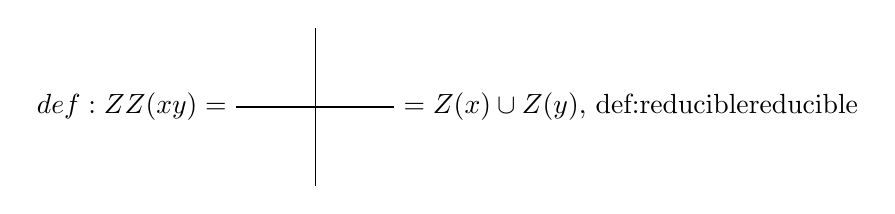
\begin{tikzpicture}
        \node [left] at (-1, 0) {$\hyperlink{def:Z}{Z}(xy)=$};
        \draw (-1, 0) -- (1, 0);
        \draw (0, -1) -- (0, 1);
        \node [right] at (1, 0) {$=Z(x) \cup Z(y)$, \hyperlink{def:reducible}{reducible}};
    \end{tikzpicture}
    \end{center}
    Also,
    \begin{center}
        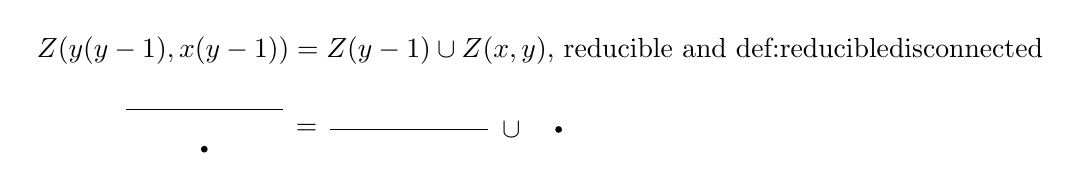
\begin{tikzpicture}
            \node [right] at (-2.25, 1) {$Z(y(y-1), x(y-1))=Z(y-1)\cup Z(x,y)$, reducible and \hyperlink{def:reducible}{disconnected}};
            \draw (-1, 0.25) -- (1, 0.25);
            \filldraw (0, -0.25) circle (1pt) {};
            \node at (1.3, 0) {$=$};
            \draw (1.6, 0) -- (3.6, 0);
            \node at (3.9, 0) {$\cup$};
            \filldraw (4.5, 0) circle (1pt) {};
        \end{tikzpicture}
    \end{center}
\end{eg}
\begin{prop}
    Any \hyperlink{def:Z}{affine variety} is a finite union of \hyperlink{def:reducible}{irreducible} affine varieties.
\end{prop}
\begin{remark}
    This is very different from usual manifolds.
\end{remark}
\begin{proof}
    If not, $Y$ is not irreducible, so $Y = Y_1 \cup Y_1'$ and one of $Y_1, Y_1'$, (say $Y_1$) is not the finite union of irreducible affine varieties, so
    \begin{equation*}
        Y_1 = Y_2 \cup Y_2',\quad Y_2 = Y_3 \cup Y_3',\quad \dotsc
    \end{equation*}
    and so we get an infinite chain of affine varities $Y \supsetneq Y_1 \supsetneq Y_2 \supsetneq \dotsb$.
    But each $Y_i = Z(I_i)$ for some ideals $I_i$.  Let
    \begin{equation*}
        W = \bigcap Y_i = Z\left(\sum I_i\right) = Z(I)
    \end{equation*}
    where $I \coloneqq \sum I_i$ is certainly an ideal.
    Ideals are finitely generated, by the Hilbert basis theorem, so $I = \langle f_1, \dotsc, f_r \rangle$ for some $f_i$.
    $f_i \in I_{a_i}$ for some $a_1, \dotsc, a_r$ so $I = I_{a_1} + \dotsb + I_{a_r}$.
    Then $W = Y_{a_1} \cap \dotsb \cap Y_{a_r}$, contradicting $Y_N \subsetneq Y_{a_1} \cap \dotsb \cap Y_{a_r}$ if $N > \max(a_1, \dotsc, a_r)$.
\end{proof}
\begin{ex}
    If $Y$ is a \hyperlink{def:Z}{subvariety} of $\A^n$, then we can write $Y = Y_1 \cup \dotsb \cup Y_r$ with $Y_i$ \hyperlink{def:reducible}{irreducible}, and $r$ minimal, uniquely up to reordering.
    Call the $Y_i$ the \textbf{irreducible components} of $Y$.
\end{ex}
\begin{defi}[Prime ideal]\hypertarget{def:prime}
    A proper ideal $I$ of a ring $R$ is \textbf{prime} if $ab \in I$ for some $a, b \in R$, then either $a \in I$ or $b \in I$.
\end{defi}
\begin{prop}
    An \hyperlink{def:Z}{affine variety} $Y$ is \hyperlink{def:reducible}{irreducible} $\iff \hyperlink{def:I}{I}(Y)$ is a \hyperlink{def:prime}{prime ideal} in $\hyperlink{def:polys}{k[\A^n]} = k[x_1, \dotsc, x_n]$.
\end{prop}
\begin{eg}
    \leavevmode
    \begin{enumerate}[label=(\roman*)]
        \item $\langle x y\rangle$ is not a \hyperlink{def:prime}{prime ideal}.
        \item Exercise: Let $R$ be a UFD, $f \in R$, $f \neq 0$, then $f$ is an irreducible polynomial $\iff \langle f \rangle$ a prime ideal.
        \item Exercise: $k[x_1, \dotsc, x_n]$ is a UFD.
            Hence $Z(y^2 - x^3 + x)$ is \hyperlink{def:reducible}{irreducible}, and $Z(y-x^2)$ is irreducible.
    \end{enumerate}
\end{eg}
\begin{proof}
    If $Y = Y_1 \cup Y_2$ is reducible, $\exists p \in Y_1 \setminus Y_2$, so $\exists f \in I(Y_2)$ such that $f(p) \neq 0$.
    Similarly, $\exists q \in Y_2 \setminus Y_1$ so $\exists g \in I(Y_1)$ such that $g(q) \neq 0$.
    Then $fg \in I(Y_1) \cap I(Y_2) = I(Y)$, but $f \notin I(Y)$, $g \notin I(Y)$ so $I(Y)$ is not prime.
    \begin{center}
        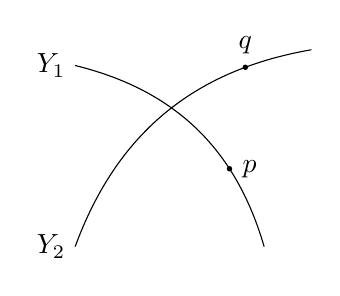
\begin{tikzpicture}
            \node [left] at (-1, 1.3) {$Y_1$};
            \node [left] at (-1, -1) {$Y_2$};
            \path (-1,1.3) edge [bend left=30] node [circle, fill, inner sep=0.7pt, pos=0.7, label=right:{$p$}] {} (1.4,-1) ;
            \path (-1,-1) edge [bend left=30] node [circle, fill, inner sep=0.7pt, pos=0.8, label=above:{$q$}] {} (2,1.5);
        \end{tikzpicture}
    \end{center}

    Conversely, if $I(Y)$ is not prime $\exists f_1, f_2 \in k[\A^n]$ such that $f_1, f_2 \notin I(Y)$ but $f_1 f_2 \in I(Y)$.
    Let \begin{equation*}Y_i \coloneqq Y \cap Z(f_i) = \set{p \in Y | f_i(p) = 0}.\end{equation*} $Y_1 \cup Y_2 = Y$, as $p \in Y \Rightarrow f_1 f_2 (p) = 0$ so either $f_1(p) = 0$ or $f_2(p) = 0$.
    Finally we must show $Y_i \neq Y$. But $f_i \notin I(Y)$, so $\exists p_i \in Y$ such that $f_i(p_i) \neq 0$ so $p_i \notin Y_i$.
\end{proof}
\begin{lemma}
    Take $X$ \hyperlink{def:reducible}{irreducible} affine \hyperlink{def:Z}{subvariety} of \hyperlink{def:affineSpace}{$\A^n$}. Then, $\mathcal{U} \subseteq X$ \hyperlink{def:zariski}{Zariski open} and non-empty $\Rightarrow \overline{\mathcal{U}} = X$.
\end{lemma}
\begin{proof}
    Let $Y = X - \mathcal{U}$, which is closed.
    Then $\overline{\mathcal{U}} \cup Y = X$, and $\mathcal{U} \neq \emptyset \Rightarrow Y \neq X$.
    But $X$ is irreducible, so $\overline{\mathcal{U}} = X$.
\end{proof}
% UP TO HERE
\color{gray}
\subsubsection*{Application: Cayley-Hamilton Theorem}
$A \in \Mat_n(k)$, an $n \times n$ matrix, with
\begin{equation*}
    \chara_A(x) = \det(x I - A) \in k[x]
\end{equation*}
the characteristic polynomial.
This gives a function $\chara_A: \Mat_n(k) \to \Mat_n(k)$ $B \mapsto \chara_A(B)$.
Cayley-Hamilton theorem says that $\forall A \in \Mat_n(k)$, $\chara_A(A) = 0$. Notice this is an equality of matrices, so it is $n^2$ equations.
\begin{proof}
    Let $X = \A^{n^2} = \Mat_n(k)$, affine space, hence irreducible algebraic variety.
    Consider $CH = \set{A \in \Mat_n(k) | \chara_A(A) = 0}$.
    Claim: this is a Zariski closed subvariety of $\A^{n^2}$, cut out by $n^2$ equations, $\chara_A(A)_y = 0$.
    We must check that these equations are polynomials in the matrix coefficients of $A$.

    %Lecture 3

    Consider $\chara_A(x) \in k[\A^{n^2 + 1}] = \det(xI - A)$, a polynomial in $x$ and in the matrix coefficients of $A$.
    \begin{equation*}
    \chara_{\begin{pmatrix}a & b//c&d\end{pmatrix}}(x) = \det
        \begin{pmatrix}
            x-a & -b \\ -c & x-d
        \end{pmatrix}
        =x^2  -(a+d) x + (ad - bc)
    \end{equation*}
    The $ij$th coefficient of $A^r$ is also a polynomial (of deg $r$) in the matrix coefficients of $A$, eg
    \begin{equation*}
        \begin{pmatrix}
            a & b \\ c & d
        \end{pmatrix}^2 =
        \begin{pmatrix}
            a^2 + bc & \dots \\
            \vdots & \ddots
        \end{pmatrix}
    \end{equation*}
    hence $\chara_A(A)_y=0$ is a poly in the matrix coefficients of $A$, proving the claim.

    Now, it is enough to prove the theorem when when $k = \overline{k}$, as $\Mat_n(k) \subseteq \Mat_n(\overline{k})$.
    Next, notice that $\chara_A(x) = \chara_{g A g^{-1}} (x)$, for $g \in \text{GL}_n$. and $\chara_A(g B g^{-1}) = g \chara_A(B) g^{-1}$ for $g \in \text{GL}_n$.
    Hence $\chara_A(A) = 0 \iff \chara_{g A g^{-1}}(g A g^{-1}) = 0$, so
    $A \in CH \iff g A g^{-1} \in CH$.
    Now, let $\mathcal{U} = \set{A \in \Mat_n(k) | A \text{ has distinct eigenvalues}}$. As $k = \overline{k}$, $A \in \mathcal{U} \implies \exists g \in \text{GL}_n$ with
    \begin{equation*}
        g A g^{-1} = \begin{pmatrix}
            \lambda_1 & 0 & \dots & 0 \\
            0 & \lambda_2 & \dots & 0 \\
            \vdots & \vdots & \ddots & \vdots \\
            0 & 0 & \dots & \lambda_n
        \end{pmatrix}
    \end{equation*}
    and it is clear that $g A g^{-1} \in CH$.
    As $k = \overline{k}$, $\#k$ is infinite, so $\mathcal{U}$ is non-empty so
    \begin{equation*}
        \emptyset \neq \mathcal{U} \subseteq CH \subseteq \A^{n^2} = X
    \end{equation*}
    hence if we show that $\mathcal{U}$ is Zariski open in $X$ then $\mathcal{U} = X$, as $X$ is irreducible. But $CH$ is closed, so $\mathcal{U} \subseteq CH$, so $CH=X$.

    Finally, we must show $\mathcal{U}$ is Zariski open.
    Observe $A \in \mathcal{U} \iff \chara_A(x) \in k[x]$ has distinct roots.
    Now recall from Galois theory, if $f(x)$ is a polynomial, $\exists$ poly $D(f)$ in the coefficients of the poly $f$ such that $f$ has distinct roots $\iff D(f) \neq 0$.

    So $A \in \mathcal{U} \iff D(\chara_A(x)) \neq 0$ is a polynomial in matrix coefficients of $A$.
\end{proof}

\color{black}
\subsection{Nullstellensatz}
Suppose $Y \subseteq \A^n$ is a subvariety,
let $I(Y) = \set{f \in k[x_1, \dotsc, x_n] | f(Y) = 0}$.
Recall we have maps
\begin{equation*}
    \begin{tikzcd}
        k[\A^n] \arrow[r] \arrow[rdd] & \{\text{functions from } k^n = \A^n \to k\} \arrow[dd] \\
                                     &\\
                         & \{\text{functions from } Y \to k\}
    \end{tikzcd}
\end{equation*}
where the composite is constructed by restricting a function from $\A^n \to k$ to $Y \to k$.
Also note that the top map is injective if $k$ is infinite.

\begin{defi}[Polynomial functions on subvariety]\hypertarget{def:kx}
    Let \begin{equation*}k[Y] \coloneqq \hyperlink{def:polys}{k[x_1, \dotsc, x_n]}/\hyperlink{def:I}{I(Y)}\end{equation*} called the \textbf{polynomial functions on $Y$}, also called \textbf{regular functions}.
\end{defi}
We just observed that $\hyperlink{def:kx}{k[Y]} \to \{\text{all functions from } Y \to k\}$ is injective if $k$ is infinite.
We've also seen $Y$ \hyperlink{def:reducible}{irreducible} $\iff \hyperlink{def:I}{I(Y)}$ is \hyperlink{def:prime}{prime} $\iff \hyperlink{def:kx}{k[Y]}$ is an integral domain.

Now let $p \in Y$. We have a map
\begin{align*}
    k[Y] &\longrightarrow k \\
    f &\longmapsto f(p)
\end{align*}
This is a $k$-algebra homomorphism, so the kernel
\begin{equation*}
    \mathfrak{m}_p = \set{f \in k[Y] | f(p) = 0}
\end{equation*}
is an ideal.
In particular, it is a maximal ideal, since here we have $k[Y]/\mathfrak{m}_p = k$, a field.
(The homomorphism is surjective as constants go to constants).

A natural question to ask now is: are any other maximal ideals in $\hyperlink{def:kx}{k[Y]}$?
In particular, what are the possible surjective $k$-algebra homomorphisms
\begin{equation*}
    \begin{tikzcd}
        k[x_1, \dotsc, x_n] \ar[r, two heads] & L
    \end{tikzcd}
\end{equation*}
with $k \subseteq L$ and $L$ a field.

For instance, taking $k=\R$, we can take the homomorphism given by the quotient map $\R[x] \twoheadrightarrow \R[x]/\langle x^2 + 1 \rangle$.
This is surjective, and has image isomorphic to $\C$, so we have a new $k$-algebra homomorphism whose image is not just $k$.
% For example, suppose $Y = \hyperlink{def:Z}{Z(x^2+1)}$ and $k=\R$. Then $k[Y] = \frac{\R[x]}{x^2 + 1}$ is not of the above form, since it is $\C$ instead of $\R$.

Claim:
If $k$ is algebraically closed, there are no $k$-algebra homomorphisms $\hyperlink{def:kx}{k[Y]} \to k$ other than evaluating at points $p \in Y$, (so the only surjections are onto $k$), and if $k \neq \overline{k}$ the only additional homomorphisms have $L$ an algebraic extension of $k$.

\begin{remark}
    Take $\mathfrak{m} \subseteq \hyperlink{def:polys}{k[x_1, \dotsc, x_n]}$ be a maximal ideal, and take $A=k[x_1, \dotsc, x_n]/\mathfrak{m}$. Then $A$ is finite dimensional over $k \iff$ every $a \in A$ is algebraic over $k$.
\end{remark}
\begin{proof}[Proof of remark]
    ($\Rightarrow$) is clear, as $1, a, a^2, \dotsc$ can't all be linearly independent over $k$.

    ($\Leftarrow$) The images of $x_1, \dotsc, x_n$ in $A$ each satisfy an algebraic relation over $k$ and they generate $A$.
\end{proof}

\begin{thm}[Nullstellensatz, version 1]
    Let $\mathfrak{m} \subseteq \hyperlink{def:polys}{k[x_1, \dotsc, x_n]}$ be a maximal ideal, and set $A=k[x_1, \dotsc, x_n]/\mathfrak{m}$. Then $A$ is finite dimensional over $k$.
\end{thm}
\begin{cor}
    If $k$ is algebraically closed, then $k \hookrightarrow A$ is an isomorphism, i.e.\ $A \cong k$.
    That is, every maximal ideal is of the form $\mathfrak{m}= \langle x_1 - p_1, \dotsc, x_n - p_n \rangle$ for $p \in k^n$.
\end{cor}
\color{gray}
\begin{proof}
    $M$ a maximal ideal $\implies A$ a field, but if $k \subseteq \overline{k}$ that means $k = \overline{k}$ algebraic over $k$. Now let $a_i$ be the image of $x_i$ in $A$, and $M$ is as stated.
    So if $k = \overline{k}$, solutions of equations $I \longleftrightarrow$ max ideal $M \subseteq k[Y] \longleftrightarrow$ alg homomorphisms $k[Y] \to k$ and if $k \neq \overline{k}$, then they are `galois orbits of solutions over bigger fields'.
\end{proof}

% Lecture 4

We can interpret this in the case $k \neq \overline{k}$ as saying: to study solutions of algebraic equations over $K$, i.e. simultaneous zero of an ideal $I$, it is necessary to study their solutions over fields bigger than $k$, such as $\overline{k}$.
\begin{proof}
    When $k$ is uncountable: If the result is not true, $\exists t \in L\setminus k$ with $t$ transcendental over $k$. In particular, $k(t) \subseteq L$. SO $\frac{1}{t-\lambda} \in L, \forall \lambda \in k$.
    But $L$ has countable dimension over $k$ (let $V_d$ be the $k$-vector space which is the image of $\set{f \in k[x_1, \dotsc, x_n] | \deg f \leq d}$, $V_d$ is finite dimensional, $\bigcup V_d = L$).
    Now consider $\frac{1}{t-\lambda}, \dotsc, \frac{1}{t-\lambda_r}$ for $\lambda_1, \dotsc, \lambda_r \in k$ distinct. If these are linearly dependent over $k$, i.e. $\exists a_i \in k$ with $\sum \frac{a_i}{t - \lambda_i} = 0$, then clearing denominators gives a poly relation in $t$, contradicting $t$ is transcendental.
    So they are linearly independent, but there are uncountably many $\lambda \in k$, a contradiction.
\end{proof}

\color{black}
\begin{cor}
    For $k = \overline{k}$, take $I \leq k[x_1, \dotsc, x_n]$ an ideal.
    Then \begin{equation*}Z(I) \neq \emptyset \iff I \neq k[x_1, \dotsc, x_n].\end{equation*}
    More generally, for $I \leq k[Y]$, \begin{equation*}Z(I) \neq \emptyset \iff I \neq k[Y].\end{equation*}
\end{cor}
Note if $k \neq \overline{k}$, this is obviously false (for instance, $I=\langle x^2 + 1 \rangle \in \R[x]$).

\begin{proof}
    For $I \leq k[Y] = k[x_1, \dotsc, x_n]/I(Y)$, replace $I$ by its inverse image in $k[x_1, \dotsc, x_n]$ to see it suffices to prove the specific case instead of the general case.

    If $I \neq k[x_1, \dotsc, x_n]$, then $I \subseteq \mathfrak{m} \subsetneq k[x_1, \dotsc, x_n]$ for $\mathfrak{m}$ a maximal ideal, since $I$ is contained in some maximal ideal.
    But Nullstellensatz gives $Z(\mathfrak{m}) = \{p\}$ for some $p \in k^n$.
    Then $Z(I) \supseteq Z(\mathfrak{m}) = \{p\} \neq 0$.
\end{proof}

\begin{remark}
    This means any ideal of equations which aren't all the equations have a simultaneous solution.
    This is equivalent to the Nullstellensatz.
\end{remark}
\begin{defi}[Radical ideal]
    Take $R$ a ring, $J \lhd R$ an ideal.  The \textbf{radical} is
    \begin{equation*}
        \sqrt{J} \coloneqq \set{f \in R | \exists n \geq 1, f^n \in J } \supseteq J
    \end{equation*}
\end{defi}
\begin{lemma}
    $\sqrt{J}$ is an ideal.
\end{lemma}
\begin{proof}
    If $\gamma \in R$, $f \in \sqrt{J}$, then $(\gamma f)^n = \gamma^n f^n \in J$ if $f^n \in J$.
    If $f, g \in \sqrt{J}$ with $f^n \in J$, $g^m \in J$ for some $n, m$ then $(f+g)^{n+m} = \sum \binom{n+m}{i} f^i g^{n+m-i}$. Either $i \geq n$ so $f^i \in J$ or $n+m-i\geq m$ then $g^{n+m-i} \in J$, so $f+g \in J$.
\end{proof}

\begin{eg}
    \leavevmode
    \begin{enumerate}[label=(\arabic*)]
        \item $\sqrt{\langle x^n \rangle} = \langle x \rangle$ in $k[x]$.
        \item If $J$ is a prime ideal, $\sqrt{J} = J$.
        \item if $f \in k[x_1, \dotsc, x_n]$ is an irreducible, then $\langle f \rangle$ is prime as $k[x_1, \dotsc, x_n]$ is a UFD, so $\sqrt{ \langle f \rangle} = \langle f \rangle$.
    \end{enumerate}
\end{eg}
Observe also that $Z(\sqrt{J}) = Z(J)$.
\begin{thm}[Nullstellensatz, version 2]
    If $k = \overline{k}$, $I(Z(J)) = \sqrt{J}$.
\end{thm}

\color{gray}
\begin{proof}
    Let $f \in I(Z(J))$, i.e. $f(p) = 0 \forall p \in Z(J)$. We must show that $\exists n$ such that $f^n \in J$.
    Consider $k[x_1, \dotsc, x_n, t]/tf-1 \coloneqq k[x_1, \dotsc, x_n, \frac{1}{f}]$.
    Let $i$ be the ideal of this, generated by the image of $J$.
    Claim: $Z(I) = \emptyset$. Proof: If not, let $p \in Z(I)$. As $J \subseteq I$, we have $p \in Z(J)$ and so $f(p) = 0$. But $p=(p_1, \dotsc, p_n, p_t)$ with $p_t \cdot f(p_1, \dotsc, p_n) = 1$, so $f(p) \neq 0$, contradiction.
    But now the corollary to Nullstellensatz version 1 gives $I=k[x_1, \dotsc, x_n, \frac{1}{f}]$. So, $1 \in I$. But $I$ is generated by $J$, so this says $1 = \sum_1^N \gamma_i/f^i$ for some $\lambda_i \in J$, $\gamma_N \neq 0$ for some $N$.
    Clear denominators and we get
    \begin{equation*}
        f^N = \sum \tilde{\gamma_i}, \tilde{\gamma_i} \in J, i.e. f^N \in J.
    \end{equation*}
\end{proof}
\begin{remark}
    This proof uses $k[x_1, \dotsc, x_n, t]/tf-1 \twoheadleftarrow k[\A^{n+1}]$. This is $k[Y]$, where $Y = Z(tf-1) \subseteq \A^{n+1}$ and $Z(tf-1) = \set{(p, t_0) | f(p) t_0 = 1}$.
    Clearly $Y \overset{\sim}{\rightarrow} \set{p \in \A^n | f(p) \neq 0} = \A^n \setminus Z(f)$.
\end{remark}
\color{black}
We will return to this, but first deduce some consequences of Nullstellensatz version 2.
\begin{cor}
    If $k = \overline{k}$, $Z(I) = Z(J) \iff I(Z(I)) = I(Z(J)) \iff \sqrt{I} = \sqrt{J}$.
    So we have a bijection
    \begin{equation*}
        \begin{tikzcd}
            \left\{\parbox{3cm}{\centering \hyperlink{def:zariski}{Zariski closed} subvarieties of \hyperlink{def:affineSpace}{$\A^n$}}\right\}
            \ar[r, bend right, hookrightarrow, "\hyperlink{def:I}{I}", start anchor=south, end anchor=south]&
            \left\{\parbox{4cm}{\centering Ideals $I \leq k[x_1, \dotsc, x_n]$ such that $\sqrt{I}=I$}\right\}
            \ar[l, bend right, two heads, "\hyperlink{def:Z}{Z}", start anchor=north, end anchor=north] \\ \\
            \text{irreducible varieties} \ar[r, leftrightarrow] & \text{prime ideals} \\
            \text{points} \rar[leftrightarrow] & \text{maximal ideals} \\
        \end{tikzcd}
    \end{equation*}
\end{cor}
The intrinsic definition of affine varieties is a consequence (doesn't depend on the embedding of $X \hookrightarrow \A^n$).
\begin{defi}[Nilpotent]
    In a ring $R$, an element $y \in R$ is \textbf{nilpotent} if $y^n = 0$ for some $n > 0$.
\end{defi}
\begin{eg}
    In $k[x]/x^7$, $x$ is nilpotent.
\end{eg}
\color{gray}
\begin{ex}
    Let $J \leq k[x_1, \dotsc, x_n]$ be an ideal, $R = k[x_1, \dotsc, x_n]/J$. Then $J = \sqrt{J} \iff R$ has no non-zero nilpotent elements.
\end{ex}
\begin{cor}
    Let $X \subseteq \A^n$ be a Zariski closed subvariety.
    Then $k[X]$ is a finitely generated $k$-algebra with no non-zero nilpotent elements.
    As it is finitely generated, there is $k[x_1, \dotsc, x_n] \overset{\alpha}{\twoheadrightarrow}k[X]$ a surjective algebra homomorphism and no non-zero nilpotents $\iff \ker \alpha$ is a radical ideal.
\end{cor}
\begin{defi}[Affine variety, v2]
    An affine variety over a field $k$ is a finitely generated $k$-algebra with no non-zero nilpotents.
\end{defi}
Observe:
\begin{enumerate}[label=(\roman*)]
    \item if $k = \overline{k}$, this coincides with our previous definition.
    \item if $k \neq \overline{k}$, we get new examples, now $\R[x,y]/x^2 + y^2 + 1$ is an affine algebraic variety over $\R$ even though $Z(x^2 + y^2 + 1) = \emptyset$.
        Note Nullstellensatz says $\R[x,y]/x^2 + y^2 + 1$ still has lots of maximal ideals but they correspond to $\Gal(\C/\R)$ orbits of complex solutions, i.e. complex conjugate pairs.
    \item this definition does not explicitly refer to a choice of embedding $X \hookrightarrow \A^n$ (the data of a choice of algebra generators for $k[X]$).
\end{enumerate}
What is missing? We still have to define what a map of algebraic varieties is.
\begin{defi}[Morphism]
    A \textbf{morphism} of algebraic varieties $X \to Y$ is a $k$-algebra homomorphism $f^*: k[Y] \to k[X]$. Write $\Mor(X, Y)$ for the set of morphisms, and write $f$ for the morphism associated to $f^*$.
\end{defi}
Let us unpack this definition.
Write
\begin{equation*}
    k[X] = k[x_1, \dotsc, x_n] / \langle s_1, \dotsc, s_l \rangle \qquad k[Y] = k[y_1, \dotsc, y_m] / \langle r_1, \dotsc, r_k \rangle
\end{equation*}
and write $\overline{y_1}, \dotsc, \overline{y_m}$ for the images of $y_i$ in $k[Y]$.
An algebra homomorphism $f^*: k[Y] \to k[X]$ takes $\overline{y_i} \mapsto f^*(\overline{y_i})$.
Choose a poly $\Phi_i = \Phi_i(x_1, \dotsc, x_n) \in k[x_1, \dotsc, x_n]$ which mod the ideal $\langle s_1, \dotsc, s_l \rangle$ equals $f^*(\overline{y_i})$.
This defines an algebra homomorphism
\begin{align*}
    k[y_1, \dotsc, y_m] &\longrightarrow k[x_1, \dotsc, x_n] \\
    y_l &\mapsto \Phi_i(x_1, \dotsc, x_n).
\end{align*}
Now the condition that this determines an algebra homomorphism $k[Y] \to k[X]$ is the condition that $r_i(\Phi_1, \dotsc \Phi_m) = 0$ in $k[X] \quad \forall i$ i.e. the ideal $\langle r_1, \dotsc, r_l\rangle$ get sent to zero in $k[X]$.
That is, $f^*$ is the data of polynomials $\Phi_1, \dotsc, \Phi_m$ in $k[x_1, \dotsc x_n]$ such that $r_i(\Phi_1, \dotsc \Phi_m) = 0$ (and the choice of such polynomials is well defined, up to adding any element of $\langle s_1, \dotsc, s_i\rangle$).
Moreover, $f^*$ determines a map of sets $X \to Y$, denoted $f:X \to Y$, $x \mapsto (\Phi_1(x), \dotsc, \Phi_m(x))$.
So, a morphism of algebraic varieties $f: X \to Y$ is, roughly speaking, a map of sets $X = (X_1, \dotsc, X_n) \in X \longrightarrow f(x) = (\Phi_1(x), \dotsc, \Phi_m(x)) \in Y$ (where $X \subseteq \A^n$ and $Y \subseteq \A^m$) given by polynomials $\Phi_1, \dotsc, \Phi_m \in k[\A^n]$. The condition that $(\Phi_1(x), \dotsc, \Phi_m(x)) \in Y$ is the condition $r_i(\Phi_1, \dotsc, \Phi_m) = 0$.
But, we gave this definition in a way which didn't require choosing $X \hookrightarrow \A^n$ etc.

\begin{defi}[Isomorphic]
    $X$ is \textbf{isomorphic} to $Y$ if $\exists \alpha^*: k[Y] \to k[X]$, $\beta^*: k[X] \to k[Y]$ such that $\alpha^* \beta^*$ and $\beta^* \alpha^*$ are identity.
\end{defi}
\begin{eg}
    \begin{enumerate}[label=(\roman*)]
        \item $t \mapsto (t^2, t^3)$ is a morphism $\A^1 \to \A^2$.
            More generally, $\Mor(\A^1, \A^n) = k$-algebra homomorphims $k[x_1, \dotsc, x_n] \to k[t]$ is just a tuple of polys $(\phi_1(t), \dotsc, \phi_n(t)) \in k[t]^n$.
        \item Take $\Mor(X, \A^1) \ni \varphi^*$, then $\varphi^* k[t] \to k[X]$ an algebra homomorphism. $k[t]$ is the free $k$-algebra on 1 generator $t$.
            That is, to specify an algebra homomorphism $k[t] \to R$ (for any ring $R$), it is enough to say where $t$ gets mapped to, and conversely any element of $R$ determines such a homomorphism.
            So $\Mor(X, \A^1) = k[X]$.
        \item $X = \A^1$, $Y = \set{(x, y) | x^2 = y^3} = Z(x^2 - y^3)$. Consider $t \mapsto (t^3, t^2)$. This is a morphism $(t^3)^2 = (t^2)^3$.
            Exercise: Is this an isomorphism? Is $Y \cong \A^1$?
        \item Take $\chara k \neq 2$. Is there a morphism $\A^1 \to \set{(x, y) | y^2 = x^3 - x}$ (which isn't a trival map).
            Do there exist polynomials $a = a(t), b=b(t) \in k[t]$, not both constant such that $b^2 = a^3 - a$.
    \end{enumerate}
\end{eg}

% Lecture 6

If $k = \overline{k}$, we can also reconstruct $f$ as follows
% points of x \longleftrightarrow max ideals m of k[X] <-> alg homs k[X] -> k
% now observe if $f^* : k[Y] \to k[X]$ and $x \in $X$, $ev_x: k[X] \to k$.
% get an alg homo $ev_x \cdot f^* : k[Y] \to k$, so the kernel is a maixmal ideal m_y$ for some y \in Y and f(x) = y
% ex: check f(x) = y

\begin{prop}
    Let $X$ be an affine algebraic variety, and $f \in k[X]$.  Then set \begin{equation*}Y = \set{(p, t) \in X \times \A^1 | t f(p) = 1}\end{equation*}.
    This is an affine algebraic variety, and the map $Y \hookrightarrow X$ with $(p, t) \mapsto p$ is a morphism of affine algebraic varieties.
\end{prop}
\begin{proof}
    It is $k[X] \to k[Y] \eqqcolon k[X][t]/tf-1$. Exercise: $k[Y]$ has no non-zero nilpotents.
\end{proof}
This means you should think of $Y \xrightarrow{\sim} X \setminus Z(f) \hookrightarrow X$.
That is, you should think of this as saying the Zariski open $X \setminus Z(f)$ is also an affine algebraic variety and the inclusion map $Y \hookrightarrow X$ is a morphism of algebraic varieties.

\begin{warning}
    Take $\set{(x, y) \in \A^2 | (x, y) \neq (0, 0)}$. This is Zariski open in $\A^2$ as $\{(0, 0)\}$ is a closed set. But, this is not an affine algebraic variety.
\end{warning}

\clearpage
\color{black}
\section{Projective space}
We will define it first as a set, then as an algebraic variety (but not an affine one).
Take $V$ a vector space over $k$ and $\dim V = n+1$ for $n \geq 0$.
\begin{align*}
    \mathbb{P}V = \mathbb{P}^n &= \{\text{set of lines through } 0 \text{ in } V\} \\
                               &= (V \setminus \{0\}) /k^\times
\end{align*}
That is, if $v \in V$, $v \neq 0$ then $k v = \set{\lambda v | \lambda \in k}$ is a line through $0$, and conversely if $l \in \mathbb{P}V$ is a line, $l = kv$ for any $v \in l \setminus 0$.

Choose a basis $e_0, \dotsc, e_n$ of $V$, write $V \overset{\sim}{\leftarrow} k^{n+1}$, $\sum x_i e_i \mapsfrom (x_0, \dotsc, x_n)$.
If $(x_0, \dotsc, x_n) \neq (0, \dotsc, 0)$, write $[x_0: \dotsc: x_n]$ for the corresponding point in $\mathbb{P}^n$ so $[\lambda x_0: \dotsc: \lambda x_n] = [x_0: \dotsc : x_n]$.

\begin{lemma}
    $\mathbb{P}^n = \A^n \sqcup \mathbb{P}^{n-1}$.
\end{lemma}
\begin{proof}
    Consider $[x_0 : \dotsc : x_n] \in \mathbb{P}^n$. Either $x_n = 0$ or $x_n \neq 0$.

    If $x_n = 0$, $p = [x_0 : \dotsc : x_{n-1} : 0]$, and $p = p' = [x_0' : \dotsc : x_n']$ if and only if $x_n' =0$ and $\lambda(x_0, \dotsc, x_{n-1}) = (x_0', \dotsc, x_{n-1}')$ for some $\lambda \in k^\times$, i.e.\ $p = p' \in \mathbb{P}^{n-1}$.

    If $x_n \neq 0$, then we can rescale $(x_0, \dotsc, x_n) = x_n \cdot (\frac{x_0}{x_n}, \dotsc, \frac{x_{n-1}}{x_n}, 1)$, so
    \begin{equation*}\set{p \in \mathbb{P}^n | x_n \neq 0} \simeq \A^n,\end{equation*}
    using the map sending
    \begin{equation*}[x_0 : \dotsc : x_n] \to \left(\frac{x_0}{x_n}, \dotsc, \frac{x_{n-1}}{x_n}\right).\end{equation*}\qedhere
\end{proof}
\begin{eg}
    \textbf{picture missing}
    \begin{equation*}\mathbb{P}^1 = \A^1 \sqcup \{\infty\}\end{equation*}
    \begin{equation*}
        \mathbb{P}^2 = \A^2 \sqcup \mathbb{P}^1 = \A^2 \sqcup \A^1 \sqcup \A^0
    \end{equation*}
    If $k = \F_q$, the number of points in $\mathbb{P}^n$ is $1 + q + \dotsc + q^n = \frac{q^{n+1}-1}{q-1}$.
\end{eg}
To phrase the above lemma without coordinates, choose $H \leq V$ a vector subspace of codimension 1, and $w_0 \in V \setminus H$.
For instance, we could use $H = \set{(x_0, \dotsc, x_n) \in V | x_n = 0}$ and $w_0 = (0, 0, \dotsc, 0, 1)$.
Then we have maps

\begin{equation*}
    \begin{tikzcd}[row sep=tiny]
        \proj H \rar[hook] & \proj V & H \lar[hook'] \\
        kv \rar[mapsto] & k v \\
                        & k(w_0 + h) \rar[mapsfrom] & h
    \end{tikzcd}
\end{equation*}
This gives $\mathbb{P}V \setminus \mathbb{P}H \xleftarrow{\sim} H$, in particular $\mathbb{P}V \setminus \mathbb{P}H \simeq \A^n$.
So the decomposition $\mathbb{P}V = \mathbb{P}H \sqcup$ (a space isomorphic to $\A^n$) depends only on the choice of a hyperplane $H$ but the isomorphism $\A^n \to \mathbb{P}V \setminus \mathbb{P}H$ depends on the choice of $w_0 \in V \setminus H$.
\begin{ex}
How does changing $w_0$ to $w_0'$ change the isomorphism?
\end{ex}

% Lecture 7

% picture of n=1
% disjoint union of two copies of A1 (complex) surjects onto P1, and intersection is sphere missing both poles
% similar argument for P1 where A is real, (drawing nicely because of the action)

% GLn acts transitively on (n+1) hyperplanes when things intersect

% repeat for P2, taking A real again
\textbf{Pictures missing}

% From this, $P^2 \twoheadleftarrow U_0 \sqcup U_1 \sqcup U_2$.
Define
\begin{align*}
    H_i       &= \set{(x_0, \dotsc, x_n) | x_i = 0} \subset k^{n+1} \\
    \proj H_i &= \set{ x\in \proj^n | x_i = 0} \\
    U_i       &= \set{x \in \proj^n | x_i \neq 0} = \proj^n \setminus \proj H_i
\end{align*}
We have
\begin{equation*}U_i \cap U_j = \set{[x_0:\dotsm:x_n] | x_i \neq 0, x_j \neq 0} \cong \A^{n+1} \times (\A^1 \setminus \{0\}).\end{equation*}
The congruence here follows by embedding $U_i \cap U_j \hookrightarrow U_i$; the image is points where $x_j/x_i \neq 0$.
In particular,
\begin{equation*}
    \begin{tikzcd}[row sep=small]
        U_i \rar["~"] & \A^n \\
        x \rar[mapsto] & \left(\dfrac{x_0}{x_i}, \dotsc, \dfrac{x_n}{x_i}\right)
    \end{tikzcd}
\end{equation*}
where $1=x_i/x_i$ is omitted.
So, this lets us see projective space as covered by open sets (analogous to charts on a manifold).
% finitary data
% done in the handout apparently
\begin{defi}
    $X \subseteq \proj^n$ is Zariski closed if $X \cap U_i$ is Zariski closed in $U_i\simeq \A^n$ for each $i=0, \dotsc, n$.
\end{defi}
Recall $E_0 = \set{(x, y) \in \A^2 | y^2 = x^3 - x}$. Sit this inside $\proj^2$ with coordinates $[X:Y:Z]$ by considering the map
\begin{equation*}
    \begin{tikzcd}[row sep=tiny]
        U_2 = \set{[X:Y:Z] | Z \neq 0} \subseteq \proj^2 \rar["~"] & \A^2 \\
        {[X:Y:Z]} \rar[mapsto] & (X/Z, Y/Z)
    \end{tikzcd}
\end{equation*}

So, the inverse gives $x = \frac{X}{Z}$ and $y=\frac{Y}{Z}$.
The equation $y^2 = x^3 - x$ becomes
\begin{align*}
    Y^2/Z^2 &= X^3 / Z^3 - X/Z \\
    \implies Y^2 Z &= X^3 - XZ^2 \qquad (\text{for } Z \neq 0)
\end{align*}
Hence,
\begin{equation*}
E_0 = \set{[X:Y:Z] | Y^2 Z = X^3 - X Z^2, Z \neq 0} \in \proj^2.
\end{equation*}

% complement of three lines, so chart Y!=0 needs to miss out third line
\begin{itemize}[label=--]
    \item On the chart $Z \neq 0$, we have the original equation $y^2 = x^3 - x$.
    \item On $Y \neq 0$, take $x = \frac{X}{Y}$, $z = \frac{Z}{Y}$, i.e. set $Y=1$, get $z = x^3 - xz^2$ for $z \neq 0$.
    \item For the chart $X \neq 0$, take $y = Y/X$, $z = Z/X$ get $y^2 z = 1 - z^2$ and $z \neq 0$.
\end{itemize}
So now take the closure of $E^0$ in $\proj^2$, which means ignore the condition $z \neq 0$. What, if any, extra points have we added?
On the chart $Y \neq 0$, if $Z = 0$ get $x^3 = 0$ the unique extra point $[0:1:0]$ % adding Z=0, Y!=0 back in gave one extra point
On the chart $X \neq 0$, if $Z=0$ get $1 = 0$, no solutions, so no extra points are added.
So, the closure of $E^0$ is $E_0 \sqcup *$, just as we wanted.

More generally, if we have $I \leq k[x_1, \dotsc, x_n]$ an ideal, $Z = Z(I) \subseteq \A^n$, we can ask what the closure of $Z$ is in $\proj^n$ using $\A^n \to \proj^n$ given by $(x_1, \dotsc, x_n) \mapsto [1:x_1:\dotsm:x_n]$.

\begin{defi}\hypertarget{def:homPoly}
    $f \in k[x_0, \dotsc, x_n]$ is \textbf{homogeneous} of degree $d$ (for $d \geq 0$) if
    \begin{equation*}
        f = \sum a_{i_0, \dotsc, i_n} x_0^{i_0} \dotsm x_n^{i_n}
    \end{equation*}
\end{defi}
If $k$ is infinite, this is equivalent to $f(\lambda x) = \lambda^df(x)$ $\forall \lambda \in k^\times$.

As we saw in the example, given $f \in k[x_1, \dotsc, x_n]$ make $f$ homogeneous:
If $\deg f = d$, define $\tilde{f}(x_0, \dotsc, x_n) = x_0^d f(x_1/x_0, \dotsc, x_n/x_0)$ and then $\tilde{f}(1, x_1, \dotsc, x_n) = f(x_1, \dotsc, x_n)$ and $\tilde{f}(\lambda x_0, \dotsc, \lambda x_n) = \lambda^d \tilde{f}(x_0, \dotsc, x_n)$ $\forall \lambda \in k^\infty$ homogeneous of degree $d$.
For example, if $f = y^2 - x^3 + x$, $\tilde{f} = z^3 ((y/z)^2 - (x/z)^3 + (x/z))$ as in our example.
Define $\tilde{0} = 0$.
Observe
(i) if $f \neq 0$, then $x_0 \nmid \tilde{f}$, and conversely
(ii) if $x_0 \nmid g$, $g \in k[x_0, \dotsc, x_n]$ which is homogeneous of degree $d$, then $\tilde{g}(1, x_1, \dotsc, x_n) = g$.
\begin{defi}
    If $I \leq k[x_1, \dotsc, x_n]$ an ideal, define $\tilde{I} = \langle \tilde{f} | f \in I \rangle$ the ideal generated by the $\tilde{f}$.
\end{defi}
% important warning
\begin{warning}
    If $I = \langle f_1, \dotsc, f_r \rangle$ it need not be the case that $\tilde{I} = \langle \tilde{f_1}, \dotsc, \tilde{f_r}\rangle$
\end{warning}
\begin{eg}
    (i) Take $I = \langle x - y^2, y \rangle$. Note this is $\langle x, y \rangle$ and so the zero set is $\{0\}$. Now, $\langle \widetilde{x - y^2}, \tilde{y} \rangle = \langle xz - y^2, y \rangle = \langle xz, y\rangle$ but $\tilde{I} = \langle \tilde{x}, \tilde{y} \rangle = \langle x, y \rangle$.
    (ii)  Can you find an example of $I$ where $\tilde{I} \neq \langle \tilde{f_1}, \dotsc, \tilde{f_r} \rangle$ for any choice of $\langle f_1, \dotsc, f_r \rangle = I$ which has $r$ minimal.
\end{eg}

% Lecture 8
Notice that every polynomial $f\in k[x_0, \dotsc, x_n]$ can be written uniquely as $f = f_{(0)} + f_{(1)} + \dotsc$ where $f_{(i)}$ is homogeneous of degree $i$.
\begin{defi}
    An ideal $I$ is homogeneous if whenever $f \in I$, then $f_{(d)} \in I$ for all $d$.
\end{defi}
\begin{eg}
    $I = \langle x y + x^2, y^3 , x^2 \rangle$ is homogeneous (follows from following lemma) while $\langle x y + y^3 \rangle$ is not.
\end{eg}
\begin{lemma} \leavevmode
    \begin{enumerate}[label=(\roman*)]
        \item $I \leq k[x_0, \dotsc, x_n]$ is homogeneous $\iff I$ is generated by a finite set of \hyperlink{def:homPoly}{homogeneous} polynomials.
        \item Suppose $k$ is infinite. $\tilde{Z} = Z(I)$ is Zariski clsoed and invariant under multiplication by $k^\times$ i.e. $p \in \tilde{Z} \iff \lambda p \in \tilde{Z}, \quad \forall \lambda \in k^\times$ if and only if $I = I(\tilde{Z})$ is a homogeneous ideal.
    \end{enumerate}
\end{lemma}
\begin{proof}
    (i) $\Rightarrow$. $I$ is generated by some polynomials $g_1, \dotsc, g_n$. If $I$ is homogeneous, then the homogeneous parts $g_{i(j)}$ are in $I$, and they generate $I$. \\
    $\Leftarrow$. If $I = \langle g_1, \dotsc, g_n \rangle$, $g_i$ homogeneous of degree $d_i$.
    Let $h \in I$, so $h = \sum f_i g_i$.
    We have to show that $h = \sum h_{(d)}$ has each piece $h_{(d)} \in I$.
    But write $f_i = \sum f_{i,(k)}$, each $f_{i,(k)}$ homogeneous of degree $k$.
    Then regroup the sum $\sum f_{i, (k)} g_k$ as $h_{(d)} = \sum_{i : \deg(g_i) = d-k} f_{i, (k)} g_i \in I$.

    (ii) $\Leftarrow$. If $I = \langle g_1, \dotsc, g_n$ with $g_i$ homogeneous of degree $d$, then $g_i (\lambda p) = \lambda^{d_i} g_i(p) = 0$ if $g_i(p) = 0$, so $\tilde{Z}$ is invariant under $k^\times$. \\
    $\Rightarrow$. The group $k^\times$ acts on $k[x_0, \dotsc, x_n]$ as algebra automorphisms $\lambda * x_i = \lambda x_i$, with $(\lambda * f) (x_0, \dotsc, x_n) = f(\lambda x_0, \dotsc, \lambda x_n)$ and $Z(I)$ is $k^\times$ stable $\iff I$ is preserved by this action.
    That is, $f \in I \implies \lambda * f \in I$.
    So, let $f \in I$, $f = f_{(0)} + f_{(1)} + \dotsb$ with $\deg f_{(i)}  = i$. We must show $f_{(i)} \in I$.
    But $\lambda * f = f_{(0)} + \lambda f_{(1)} + \lambda^2 f_{(2)} + \dotsb$ so if we pick $\lambda_0 = 1$, $\lambda_1, \dotsc, \lambda_n \in k^\times$.
    \begin{align*}
        f = &\lambda_0 * f = f_{(0)} + f_{(1)} + f_{(2)} + \dotsb + f_{(n)} \\
            &\lambda_1 * f = f_{(0)} + \lambda_1 f_{(1)} + \lambda_1^2 f_{(2)} + \dotsb + \lambda_1^n f_{(n)} \\
        \vdots
            &\lambda_n * f = f_{(0)} + \lambda_n f_{(1)} + \lambda_n^2 f_{(2)} + \dotsb + \lambda_n^n f_{(n)} \\
    \end{align*}
    That is,
    \begin{equation*}
        \begin{pmatrix}
            1 & 1 & \dots & 1 \\
            1 & \lambda_1 & \dots & \lambda_1^n \\
            \vdots & \vdots & \ddots & \vdots \\
            1 & \lambda_n & \dots & \lambda_n^n \\
        \end{pmatrix}
        \begin{pmatrix}
            f_{(0)} \\f_{(1)} \\ \vdots \\f_{(n)}
        \end{pmatrix}
        =
        \begin{pmatrix}
            \lambda_0 \\ \lambda_1 \\ \vdots \\ \lambda_n
        \end{pmatrix}
        * f
    \end{equation*}
    So if we choose $\lambda_i \neq \lambda_j$ for all $i \neq j$ (possible as $\#k$ infinite), the determinant is
    \begin{equation*}
        \pm \prod_{i < j} (\lambda_i - \lambda_j) \neq 0
    \end{equation*}
    so we can invert the matrix and write $f_{(d)}$ as a linear combination of $\lambda_0 * f, \dotsc, \lambda_n * f$ all of which are in $I$.
    Hence $I$ is a homogeneous ideal.
\end{proof}
Recall $V = \A^{n+1}$, $H \leq \A^{n+1}$ a hyperplane, e.g.\ $H = \{x_0 = 0\}$, pick $p_0 \in V \setminus H$.
\begin{equation*}
    \A^n= \proj V \setminus \proj H \hookrightarrow \proj^n = \proj V
\end{equation*}
% (***) on the hook right arrow
$Z = Z(I) \subseteq \A^n \leadsto \tilde{I}$ a homogeneous ideal in $n+1$ variables, which generated the closure of $Z$ inside $\proj^n$.
In particular, the homogeneous ideal can be seen as defining a closed subvariety $\tilde{Z}$ of $\A^{n+1}$ such that $p \in \tilde{Z}$, then $\lambda p \in \tilde{Z} \; \forall \lambda \in k^\times$.
This corresponds to a closed subvariety of $\proj^n$ where $l \in $subvariety $\iff l = k p = \langle p \rangle$ for $p \in \tilde{Z}$, $p \neq 0$.
If $k = \overline{k}$, Nullstellensatz says this subvariety $\subseteq \proj^n$ is non-empty.
\begin{equation*}
    \iff \tilde{Z} \supseteq \{(0)\} \iff \text{ homogeneous ideal } I \lneq \langle x_0, \dotsc, x_n \rangle
\end{equation*}
i.e.\ Zariski closed subvarieties of $\proj^n \leftrightarrow$ homogeneous ideals in $x_0, \dotsc, x_n$ different from $\langle x_0, \dotsc, x_n \rangle$.
\begin{ex}
    Show that (***) defines a bijection
    % closed varieties of A^n <-> closed subvarities \overline{Z} of Pn such that no irreducible component of \overline{Z} is contains in \proj V \setminus \A^n = \proj H
    % Z \mapsto \overline{Z} = closure of I(Z) in \proj V
\end{ex}
\begin{defi}
    A projective variety is a closed subvariety of $\proj^n$, some $n$
\end{defi}
An affine variety is $k[X] = k[x_1, \dotsc, x_n]/I$, $I = \sqrt{I}$.
\begin{defi}
    A quasi-affine variety is an open subvariety of an affine variety
    A quasi-projective variety is an open subvariety of a projective variety.
\end{defi}
\begin{ex}
    If $\mathcal{U} \subseteq X$ an open subset of a variety $X$, $\exists$ structure of a variety on $\mathcal{U}$ makes the embedding a morphism of varieties.
\end{ex}

% Lecture 9
\section{Smooth points, dimension, Noether normalisation}
Let $X \subseteq \A^n$ be an affine variety, $p \in X$. Write $X = Z(I)$, $I = \langle f_1, \dotsc, f_r \rangle$.
We would like to think about the tangent space to $X$ at $p$, a vector space.
Our tentative definition is
\begin{align*}
    T_p X &= \Set{v \in \A^n | \sum v_i \frac{\partial f_j}{\partial x_i}(p) = 0, j = 1,\dotsc, r} \\
    &= \Set{v \in \A^n | \sum v_i \frac{\partial f}{\partial x_i}(p) = 0, \forall f \in I}
\end{align*}
For example, take $I = \langle y^2 - x^3 \rangle$.
% pic
Then
\begin{equation*}
    T_{(p_1, p_2)} X = \Set{(v_1, v_2) | v_1 (-3p_1^2) + v_2 (2 p_2) = 0}.
\end{equation*}
So if $(p_1, p_2) \neq (0, 0)$ then $T_{(p_1, p_2)} X$ is a line, and if $(p_1, p_2) = (0, 0)$ then $T_{(p_1, p_2)} X = \A^2$.
\begin{remark}
    You can think of $T_p X$ as sitting at $p \in X$, by translating $v \mapsto v + p$.
    So,
    \begin{equation*}
        T_p X \simeq \set{v \in \A^n | \sum_i (v_i - p_i) \frac{\partial f}{\partial x_i} (p) = 0, \forall f \in I}.
    \end{equation*}
    We can think of this as a linear approximation to the variety:
    \begin{equation*}f(x) = f(p) + \sum_i (x - p_i) \frac{\partial f}{\partial x_i} + \text{ higher order terms}.\end{equation*}
\end{remark}
\begin{lemma}
    \begin{equation*}
        \set{p \in X | \dim T_p X \geq d}
    \end{equation*}
    is a Zariski closed subvariety of $X$, for all $d \geq 0$.
\end{lemma}
\begin{proof}
    Let $X = Z(I)$, where $I = \langle f_1, \dotsc, f_r \rangle$. Then write
    \begin{equation*}
        T_p X = \ker A, \quad
        A =
        \begin{pmatrix}
            \frac{\partial f_1}{\partial x_1} & \dots & \frac{\partial f_1}{\partial x_n} \\
            \vdots & \ddots & \vdots \\
            \frac{\partial f_r}{\partial x_1} & \dots & \frac{\partial f_r}{\partial x_n} \\
        \end{pmatrix}
    \end{equation*}
    where $A: k^n \to k^r$ is a linear map.
    Recall $\dim(\ker A) + \text{rank}(A) = 0$ by the rank-nullity theorem.  So,
    \begin{align*}
        \dim \ker A \geq d &\iff n - \text{rank} A \geq d \\&\iff \text{rank} A \leq n - d.
    \end{align*}
    But the rank of a matrix is greater than $a$ if and only if there exists some $a \times a$ submatrix with non-zero determinant.
    So, $\text{rank}(A) \leq d \Leftrightarrow \text{all } (n - d + 1) \times (n - d + 1)$ subminors have zero determinant which is a collection of polynomial equations.
    That is,
    \begin{equation*}I (\set{p \in X | \dim T_p X \geq d}) = \langle f_1, \dotsc, f_r, \text{ determinants of all subminors} \rangle.\end{equation*}
\end{proof}
The problem with the definition from earlier was that it depends on an embedding, and we want a definition of $T_p X$ which doesn't depend on embedding $X \hookrightarrow \A^n$.
\begin{defi}\hypertarget{def:derivation}
    Take $A$ an algebra over $k$, and $\varphi: A \to k$ a homomorphism. (For example, consider $A = k[X]$, $\varphi = \text{ev}_p: f \mapsto f(p)$.)

    A \textbf{derivation} `centered at $\varphi$' is a $k$-linear map $D: A \to k$ such that
    \begin{equation*}
        D(fg) = D f \varphi (g) + \varphi(f) Dg \tag{Leibniz rule}
    \end{equation*}
    Write $\Der(A, \varphi)$ for the set of such derivations, a vector space over $k$.
\end{defi}
\begin{eg}
    Take $A = k[x_1, \dotsc, x_n]$, $p \in \A^n$.
    If $(v_1, \dotsc, v_n) \in \A^n$, then $D(f) = \sum v_i \frac{\partial f}{\partial x_i} (p)$ is a \hyperlink{def:derivation}{derivation} centered at $\text{ev}_p$.
    Moreover, it is the unique derivation with $D(x_i) = v_i$. Exercise: Show it is unique.

    Conversely, given $D \in \Der(A, \dotsc, x_n], ev_p)$, we get $v_i = D(x_i)$ so $\Der(A, \text{ev}_p) = T_p \A^n$.
\end{eg}
More generally,
\begin{lemma}
    Let $A = \hyperlink{def:polys}{k[x_1, \dotsc, x_n]}/\langle f_1, \dotsc, f_r \rangle = k[X]$ and take $p \in X$.
    \begin{align*}
        \Der(A, \text{ev}_p) &= \Set{D = \sum_i v_i \frac{\partial}{\partial x_i}\Big\rvert_p | D \langle f_1, \dotsc, f_r \rangle = 0 \text{ in } k[X]} \\
                             &= \Set{D = \sum_i v_i \frac{\partial}{\partial x_i}\Big\rvert_p | \sum_i v_i \frac{\partial f_j}{\partial x_i}(p) = 0 \ \forall j}
    \end{align*}
\end{lemma}
\begin{proof}
    Can be seen as above.
    Alternatively, $D \in \Der(k[X], \text{ev}_p)$ determines $\tilde{D} \in \Der(k[x_1, \dotsc, x_n], \text{ev}_p)$ and then the condition $\tilde{D}$ descends to a map $k[X] \to k$ is the condition $D\langle f_1, \dotsc, f_r \rangle = 0$.
    % more details?
\end{proof}
This gives us a better definition of tangent space:
\begin{defi}[Intrinsic definition of tangent space]
    \begin{equation*}
        T_p X = \Der(k[X], \text{ev}_p).
    \end{equation*}
\end{defi}
We can almost immediately conclude that this gives a definition for any algebraic variety.
\begin{ex}
    Let $V = X \setminus Z(f)$, for $f \in k[X]$ be a Zariski open affine subvariety of $X$, i.e.\
    \begin{equation*}
        k[V] = k[X]\left[\frac{1}{f}\right].
    \end{equation*}
    Show that $T_p V \cong T_p X$ under a canonical isomorphism, i.e.\ that
    \begin{equation*}\Der\left(k[X]\left[\frac{1}{f}\right], \text{ev}_p\right) \xrightarrow{\sim} \Der(k[X], \text{ev}_p)\end{equation*}
    for $f(p) \neq 0$.
\end{ex}
So now $T_p X = T_p U$, for $U$ any Zariski open subvariety: the tangent space is Zariski local.
% pic

\begin{eg}
    Take $X = \proj^n$, $p = [p_0: p_1: \dotsb: p_n]$. If $p_0 \neq 0$, $p = [1: \frac{p_1}{p_0} : \dotsb : \frac{p_n}{p_0}] = \iota(\bar{p})$, the embedding of some $\bar{p} \in \A^n \hookrightarrow \proj^n$. Then
    \begin{equation*}
        T_p \proj^n = T_{\bar{p}} \A^n = \A^n.
    \end{equation*}
\end{eg}
\begin{defi}
    Let $X$ be irreducible. Then the \textbf{dimension} of $X$:
    \begin{equation*}
        \dim X \coloneqq \min \set{\dim T_p X | p \in X}
    \end{equation*}
\end{defi}
\begin{eg}
    $\dim A^n = n = \dim \proj^n$, $\dim \set{(x, y) | y^2 = x^3} = 1$.
\end{eg}
If $X$ is not irreducible, the dimension is not such a great concept.
\begin{defi}
    If $X$ is arbitrary, $\dim X \coloneqq \max\set{\dim X_i | X_i \text{ a \hyperlink{def:component}{component} of } X}$.
\end{defi}
\begin{defi}
    If $X$ is irreducible, $p \in X$ is \textbf{smooth} if $\dim T_p X = \dim X$, and singular otherwise and we've shown singular points in $X$ form a Zariski closed subvariety, whose complement is non-empty. % (lemma from earlier in lecture)
\end{defi}
\begin{lemma}
    Let $f \in k[x_1, \dotsc, x_n]$ be prime. Then $\dim Z(f) = n-1$. Call this a `hypersurface'.
\end{lemma}
\begin{proof}
    $T_p Z(f)$ has dimension $n$ or $n-1$, and $T_p Z(f) = \A^n \iff \forall i \, \frac{\partial f}{\partial x_i} = 0$.
    So $T_p Z(f)$ has dimension $n$ for all $p \in Z(f) \implies \frac{\partial f}{\partial x_i} \in I(Z(f)) \quad \forall i=1, \dotsc, n$.
    But $I(Z(f)) = \sqrt{f}$, by Nullstellensatz, so $=(f)$ as $f$ is prime.
    So, $\frac{\partial f}{\partial x_i} = f . g$ for some $g$. But $\deg x_i \frac{\partial f}{\partial x_i} < \deg_{x_i} f \implies g = 0$.
    So $\dim Z(f) = 0 \implies \frac{\partial f}{\partial x_i} = 0 \quad \forall i$.
    There are now two cases,
    \begin{enumerate}[label=(\roman*)]
        \item if $\chara k = 0$, this implies $f = 0$.
        \item if $\chara k = p$, this implies $f \in k[x_1^p, \dotsc, x_n^p]$ as $\frac{\partial (x^p)}{\partial x} = p x^{p-1} = 0$.
    \end{enumerate}
    Claim: $\exists g \in k[x_1, \dotsc, x_n]$ such that $g(x)^p = f(x)$.
    Proof: If $f = \sum a_\lambda x^{\lambda p}$, $g = \sum a_\lambda^{1/p} x^\lambda$ (for $a_\lambda \in k$) which requires can take $p$th roots of things in $k$, which is allowed if $k = \bar{k}$.
    But this contradicts $f$ is prime!
\end{proof}
% Lecture 10
There are two other notions of dimension:
\begin{enumerate}[label=(\arabic*)]
    \item Krull dimension:
        \begin{equation*}
            \dim_{Kr} X = \max\set{r | \emptyset \neq Z_0 \lneq Z_0 \lneq Z_1 \lneq \dotsb \lneq Z_r = X}
        \end{equation*}
        where each $Z_i$ is an irreducible Zariski closed subvariety.

        For example, take $\A^1$. The only such chains are $\text{point} \lneq \A^1$, so $\dim_{Kr} \A^1 = 1$.
        We won't have time show show $\dim_{Kr} X = \dim X$.
    \item If $X$ is affine and irreducible, define $k(X)$ as the field of fractions of $k[X]$, which is non-zero as $k[X]$ is an integral domain.
        This is
        \begin{align*}
            k(X) &= \set{f/g | f, g \in k[X]} \\
                 &= \bigcup_{g \in k[X]} k[X \setminus Z(g)] \\
                 &= \bigcup_{g \in k[X]} k[X][\frac{1}{g}] \\
                 &= \bigcup_{U \subseteq X} \text{Zar. open, affine} k[U]
        \end{align*}
        called the function field of $X$.
        Observe that if $U \subseteq X$ is affine and open, then $k(U) = k(X)$.
        But this means that if $X$ is any irreducible variety, affine or not, can define $k(X) = k(U)$, for $U$ any affine open subset of $X$.

        Examples:
        \begin{enumerate}[label=(\roman*)]
            \item $k(\A^n) = k(x_1, \dotsc, x_n)$
            \item $k(\proj^n) = k(\frac{x_1}{x_0}, \dotsc, \frac{x_n}{x_0}) \simeq k(\frac{x_0}{x_n}, \dotsc, \frac{x_{n-1}}{x_n})$ since $\frac{x_i}{x_0} \cdot \frac{x_0}{x_n} = \frac{x_i}{x_n}$.
            \item if $E = \set{(x, y) | y^2 = x^3 - x}$, then $k(E) = k(x)[y]/\langle y^2 = x^3 - x \rangle$
            \item $X = \set{(x, y) | y^2 = x^3}$, $k(X) = k(x)[y] / \langle y^2 = x^3 \rangle$
        \end{enumerate}

        Now we can define $\text{trdim} X =$ the transcendance dimension of extension $k \subseteq k(X)$.
        We need a small lemma to show trdim $k(x_1, \dotsc, x_n)/k = $ trdim $\A^n$ = n.
\end{enumerate}
\begin{thm}
    For any algebraic variety $X$ trdim $X = \dim X$.
\end{thm}
Proof strategy: We will reduce this to $\A^n$ where we know $\dim \A^n = n = \text{trdim} \A^n$ by looking for very special nice morphisms $X \to \A^n$.
To motivate this, consider the following special situation.
Suppose $k = \overline{k}$ and take a morphism $\varphi: X \to Y$ of affine varieties such that
\begin{enumerate}[label=(\arabic*)]
    \item $X, Y$ are irreducible
    \item \begin{equation*}
        k[X] = k[Y][t]/\langle f(t) \rangle
        \end{equation*}
        and $\varphi$ is the inclusion $k[Y] \hookrightarrow k[Y][t]/\langle f\rangle = k[X]$ where $f(t) \in k[Y][t]$,
        \begin{equation*}
            f(t) = a_0(y) + a_1(y)t + \dotsb + a_N(y) t^N = f(y, t) \quad \text{with } a_N \neq 0
        \end{equation*}
    \item $f$ is a separable polynomial, when regarded as an element of $k(Y)[t]$, i.e.\
        \begin{equation*}
            F(t) = \frac{f(t)}{a_N(y)} = t^N + \frac{a_{N-1}}{a_N} t^{N-1} + \dotsb + \frac{a_0}{a_N}
        \end{equation*}
        is such that $F(t), F'(t)$ have no common roots i.e.\ $\varphi X \to Y$ comes from a separable algebraic extension of function fields $k(X) \supseteq k(Y)$.
\end{enumerate}
In this situation, we have a lemma
\begin{lemma}
    \leavevmode
    \begin{enumerate}[label=(\alph*)]
        \item $\varphi(X)$ contains an open (hence dense!) subset of $Y$
        \item exists an open non-empty subset $V \subseteq Y$ such that $\varphi^{-1}(V)$ is finite, $\# \varphi^{-1}(v) \leq N, \; \forall v \in V$.
    \end{enumerate}
\end{lemma}
\begin{proof}
    (b). $X = \set{(y_0, t_0) \in Y \times \A^1 | f(y_0, t_0) = 0}$ and the morphism $X \to Y$ sends $(y_0, t_0) \mapsto y_0$.
    Now for fixed $y_0 \in Y \setminus Z(a_N)$, $f(y_0, t)$ is a polynomial in $k[t]$ of degree $N$ so has at most $N$ roots.
    (a). Let $U = \set{y \in Y | a_N(y) \neq 0} = Y \setminus Z(a_N)$ is Zariski open.
\end{proof}
\begin{ex}
    If $f: X \to Y$ is a morphism of affine varieties then we get $\forall p \in X$, a map $df: T_p X \to T_{f(p)} Y$
\end{ex}
\begin{prop}
    In the same situation as above, exists a Zariski open $U \subseteq Y$ such that $\forall (y_0, t_0) \in X$ such that $y_0 \in U$, and the natural map $T_{(y_0, t_0)} X \to T_{y_0} Y$ is an isomorphism.
\end{prop}
\begin{proof}
    Let $Y \subseteq \A^n$, so $T_{y_0} Y = \set{v \in \A^n | \sum v_i \frac{\partial h}{\partial x_i}(y_0) = 0, \forall h \in I(Y)}$ and
    \begin{equation*}
        T_{(y_0, t_0)} X = \Set{(v, \gamma) \in \A^n \times \A^1 | \sum v_i \frac{\partial h}{\partial x_i}(y_0) = 0, \forall h \in I(Y), \text{and } \sum v_i \frac{\partial f}{\partial x_i} (y_0, t_0) + \gamma \frac{\partial f}{\partial t}(y_0, t_0) = 0}.
    \end{equation*}
    as $I(X) = \langle I(Y), f \rangle$ but this is
    \begin{equation*}
        \set{(v, \gamma) \in T_{y_0} X \times \A^1 | \sum v_i \frac{\partial f}{\partial x_i} + \gamma \frac{\partial f}{\partial t}(y_0, t_0) = 0}.
    \end{equation*}
    If $\frac{\partial f}{\partial t}(y_0, t_0) \neq 0$, then can divide by it, and get isomorphism $T_{y_0} X \overset{\sim}{\rightarrow} T_{(y_0, t_0)} X$.
    So the proposition is equivalent to $\exists$ Zariski open subset $U$ of $Y$ such that $\forall y_0 \in U \forall t_0$ with $f(y_0, t_0) = 0$, $\frac{\partial f}{\partial t}(y_0, t_0) \neq 0$.
    But this is immediate if $\frac{\partial f}{\partial t}$ isn't the zero polynomial, and our assumption of separability implies this.
\end{proof}

\begin{enumerate}[label=(\arabic*)]
    \item Note separability is necessary. For instance, take $k = \overline{\mathbb{F}_p}$, $Y = \A^1$, $X = \set{(y, t) | y = t^p}$.
        \begin{equation*}
            T_{(y_0, t_0)} X = \set{(v, \gamma)} X = \set{(v, \gamma) | v - p t_0^{p-1} \cdot \gamma = 0} = \set{(0, \gamma) | \gamma \in \A^1}
        \end{equation*}
        and map $T_{y_0, t_0} X \to T_{y_0} \A^1$ by $(0, \gamma) \mapsto 0$.
    \item $\dim X = \dim Y$, $\trdim X = \trdim Y$. The second equality is clear as this is a separable algebraic extension of fields.
        To prove the first, let $Y^{sm}$ be the smooth points of $Y$. $Y$ irreducible, so $Y^{sm} \cap U$ is open and Zariski dense. and $\dim T_p Y = \dim Y$ if $y \in Y^{sm} \cap U$.
        but $\varphi^{-1} (Y^{sm} \cap U)$ is open in $X$, so $\dim X = \dim T_{(p, t)} X$ any $(p, )$ in this set.
\end{enumerate}

Finally, note morphisms as above with $a_N = 1$, i.e.\ $f$ a monic polynomial, are even nicer. $\varphi$ is surjective.

% new lecture
Suppose we have affine varieties $X$ and $Y$ with morphism $k[X] = k[Y][t]/f(t) \leftarrow k[Y]$.
We noticed that if $f \in k[Y][t]$ is a monic polynomial, then the map of algebraic varities $X \xrightarrow{\varphi} Y$ is surjective with finite $\varphi^{-1}(y)$ $\forall y \in Y$.

\begin{defi}
    $B \subseteq A$ is an integral ring extension if $\forall a \in A$, $\exists$ a monic polynomial $f \in B[t]$ with $f(a) = 0$.
\end{defi}
\begin{lemma}
    \begin{enumerate}[label=(\roman*)]
        \item If $f$ is a monic polynomial, then $B \subseteq B[t]/\langle f(t) \rangle$ is an integral extension of $B$.
        \item If $C \subseteq B \subseteq A$ are integral ring extensions, so is $C \subseteq A$.
    \end{enumerate}
\end{lemma}
\begin{defi}
    If $\phi^*: k[Y] \to k[X]$ is an integral inclusion of rings, we say $\varphi: X \to Y$ is a \textbf{finite morphism}.
\end{defi}
\begin{thm}[Noether normalisation lemma]
    Let $X$ be an affine variety. Then there exists a finite surjective morphism $X \to \A^d$ for some $d$.
    More precisely, let $k$ be such that $\chara k = 0$ or $\chara k = p$ and $x \mapsto x^p$ is surjective, e.g.\ $k$ is finite or algebraically closed.
    Let $A$ be a finitely generated algebra over $k$ and an integral domain. Then $\exists x_1, \dotsc, x_N$ which generate $A$ as a $k$-algebra such that
    \begin{enumerate}[label=(\roman*)]
        \item $x_1, \dotsc, x_d$ algebraically independent over $k$
        \item for each $i > d$, $x_i$ is separable algebraic with monic polynomial $F_i[t] \in k[x_1, \dotsc, x_{i-1}][t]$. That is, $k[x_1, \dotsc, x_{i-1}] \subseteq k[x_1, \dotsc, x_i]$ is an integral extension for $i > d$.
    \end{enumerate}
\end{thm}
Notice, by the lemma (i) and (ii), this says that $k[x_1, \dotsc, x_d] \subseteq A$ is an integral ring extension.
\begin{cor}
    $\trdim X = \dim X$.
\end{cor}
\begin{proof}
    We showed last time $\trdim \A^d = d = \dim \A^d$, and that if $\varphi: X \to Y$ had this nice form, then $\trdim X = \trdim Y$, $\dim X = \dim Y$.
\end{proof}
\begin{eg}
    Take $k = \C$, and $X = \set{(x, y) \in \A^2 | x y = 1}$. Notice that $X \to \A^1$ with $(x, y) \mapsto x$ is not a finite morphism, as $k[x] \hookrightarrow k[x, y] /xy-1$ is not of the form $k[x][t]/(f(t))$ with $f$ monic.
    However $X \to \A^1$ given by $(t, t^{-1}) \mapsto t + t^{-1} = z$ is finite, since $z = t+t^{-1} \implies t^2 - tz + 1 = 0$, i.e.\
    \begin{equation}
        k[t, t^{-1}] = k[z][t]/t^2-tz+1
    \end{equation}
    and indeed any projection onto a line other than the $x$ or $y$ axis will work.
\end{eg}
\begin{thm}
    If $k = \overline{k}$, and $\varphi: X \to Y$ is a morphism of algebraic varities, and $X$, $Y$ irreducible.
    \begin{enumerate}[label=(\alph*)]
        \item $\overline{\varphi(X) = Y} \iff$ algebra homomorphism $k[Y] \to k[X]$ is injective.
        \item Suppose $\overline{\varphi(X) = Y}$. Then
            \begin{enumerate}[label=(\roman*)]
                \item $\dim X \geq \dim Y$
                \item there exists an open subset $U \subseteq Y$, non-empty such that $\forall y \in U$, $\dim \phi^{-1} y = \dim X - \dim Y$.
                \item For all $y \in \varphi(X)$, $\dim \varphi^{-1}(y) \geq \dim X - \dim Y$.
            \end{enumerate}
    \end{enumerate}
\end{thm}
\begin{eg}
    Take $X = \A^2 = Y$, and $\varphi: (x, y) \mapsto (xy, y)$.
    If $U = \set{(a, b) | b \neq 0}$, $\varphi^{-1}\{(a, b)\} = \{(a/b, b)\}$ a point, $\dim \varphi^{-1}(a, b) = 0 = 2- 2$.
    If $b = 0$, then
    \begin{equation}
        \varphi^{-1}((a, 0)) =
        \begin{cases}
            \emptyset & \text{if } a \neq 0 \\
            \A^1 \times \{0\} & \text{if } a = 0
        \end{cases}
    \end{equation}
    with dimension $1 > 0$. Notice $\varphi$ is not surjective but $\overline{\varphi(X)} = Y$.
\end{eg}
\begin{proof}
    \begin{enumerate}[label=(\alph*)]
        \item Let $f \in \ker(k[Y] \to k[X])$. Then $\forall x \in X$, $f \circ \varphi (x) = 0$, so $f|_{\varphi(X)} = 0$ so $f|_{\overline{\varphi(X)}} = 0$, as $f$ is continuous.
            Hence if $\overline{\varphi(X)} = y$, $f \equiv 0$ on $Y$, so $f = 0$. Converse is exercise.
        \item
            \begin{enumerate}[label=(\roman*)]
            \item $k[X]$ and $k[Y]$ are integral domains, so the fraction field $k(Y) \hookrightarrow k(X)$, hence $\trdim Y \leq \trdim X$.
            \item Claim: Noether normalisation $\implies \exists$ open subset $V \subseteq Y$, $V \neq \emptyset $ such that if you put $U = \varphi^{-1}(V)$, the map $\varphi: U \to V$ factors as $\varphi = p \circ \alpha$, for $\alpha: U \to \A^d \times V$ a finite morphism and $p: A^d \times V \to V$, $p(a, v) = v$ is projection.
                Exercise: Show the claim shows part (ii) of the proposition. Prove the claim. Hint: Let $L = k(Y)$, set $A = L. k[X] \subseteq k(X)$ be the subalgebra of $k(X)$ generated by $L$ and $k[X]$, so an algebra over the field $L$.
                Apply Noether to $A$ over the field $L$ to get $a_1, \dotsc, a_d$ in $A$ are algebraically independent over $L$, such that $A$ is integral over $L[a_1, \dotsc, a_d]$ and generated by $a_{d+1}, \dots, a_N$.
                Put $a_i$ over a common denominator and deduce the result.
            \end{enumerate}
    \end{enumerate}
                % missing stuff?
\end{proof}

Noether normalisation restate: $A$ is a finitely generated algebra over a field $k$, and an integral domain. THen there exist $x_1, \dotsc, x_d \in A$ algebraically independent over $k$, and $x_{d+1}, \dotsc, x_n \in A$ such that
\begin{enumerate}[label=(\roman*)]
    \item $x_1, \dotsc, x_n$ generate $A$
    \item for each $i > d$, $x_i$ satisfies a monic irreducible polynomial $F_i$ with coefficients in $k[x_1, \dotsc, x_{i-1}]$.
\end{enumerate}
Moreoever, if $k$ is perfect, then $F_i$ can be chosen to be separable.
\begin{defi}[Perfect]
    A field $k$ is perfect if $\chara k = p > 0$ and $x \mapsto x^p$ is a surjection.
\end{defi}
\begin{remark}
    In particular, $A \supseteq B \coloneqq k[x_1, \dotsc, x_d]$ and $B \subseteq A$ is an integral ring extension.
\end{remark}
Noether normalisation implies Nullstellensatz.
We will need a lemma:
\begin{lemma}
    If $B \subseteq A$ is an integral ring extension, then
    \begin{equation*}
        \text{units of } B = \text{units of A} \cap B
    \end{equation*}
\end{lemma}
\begin{proof}
    Let $b \in B$, and suppose $b$ has an inverse in $A$, i.e. $a \in A$ such that $ab = 1$.
    As $B \subseteq A$ is integral, $\exists c_i \in B$ such that $a^n + c_{n-1} a^{n-1} + \dotsb + c_0 = 0$, (i.e.\ $a$ satisfies a monic polynomial with coefficients in $B$).
    Now multiply by $b^{n-1}$, get $a = -c_{n-1} - c_{n-2} b - \dotsb - c_0 b^{n-1} \in B$.
\end{proof}
Recall
\begin{thm}[Nullstellensatz]
    If $A = k[z_1, \dotsc, z_n]/m$, $m$ a maximal ideal (so $A$ is a field), then all elements of $A$ are algebraic over $k$.
\end{thm}
\begin{proof}
    By Noether, $A \supseteq B = k[x_1, \dotsc, x_n]$ with $x_1, \dotsc, x_d$ algebraically independent, and $A$ integral over $B$.
    Assume $d > 0$.  The units in $B$ are just $k^\times$, for example $x_1$ is not invertible.
    Hence by the lemma, $x_1$ is not invertible in $A$. But $A$ is a field, so contradiction.
    So $d = 0$, and $A$ is integral over $B$, in particular algebraic.
\end{proof}

% \begin{note}
%     Projective $n$-space is compact. In particular, $\proj^n(\C)$
% \end{note}
\section{Algebraic Curves}
From now on assume $k = \overline{k}$.
\begin{defi}
    A \textbf{curve} is a \hyperlink{def:quasiProjVar}{quasi-projective variety} $X$ with $\dim X = 1$.
\end{defi}
For $\dim X = 1$:
\begin{align*}
    \trdim k(X) = 1 &\iff \forall p \in X \setminus \text{some finite set}, \dim T_p X = 1 \\
                    &\iff \text{only Zariski closed proper subvarieties of $X$ are finite sets of points}.
\end{align*}
\begin{eg}
    If $F = F(X_0, X_1, X_2)$, an irreducible homogeneous polynomial, then $Z(F) \subseteq \proj^2$ is an irreducible projective curve.
\end{eg}
\begin{warning}
    Not all curves can be embedded inside $\proj^2$ (in fact, most curves are not plane curves).
\end{warning}
\begin{defi}
    If $X$ is an algebraic variety, and $p \in X$. Define
    \begin{enumerate}[label=(\roman*)]
        \item $\mathcal{O}_{X, p} = \set{f / g \in k(X) | g(p) \neq 0}$, rational functions defined in some Zariski neighbourhood of $p \in X$. This is the \textbf{local ring} of $X$ at $p$.
        \item $\mathfrak{m}_{X, p} = \set{\gamma \in k(X) | \gamma(p) = 0}$ the maximal ideal of $\mathcal{O}_{X, p}$.
    \end{enumerate}
\end{defi}
\begin{ex}\leavevmode
    \begin{enumerate}[label=(\roman*)]
        \item Show if $\gamma \in \mathcal{O}_{X, p} \setminus \mathfrak{m}_{X, p}$, then $\gamma^{-1}$ exists in $\mathcal{O}_{X, p}$ hence $\mathfrak{m}_{X, p}$ is the unique maximal ideal.
        \item $\mathcal{O}_{X, p} / \mathfrak{m}_{X, p} = k$
    \end{enumerate}
\end{ex}
If $X$ is a curve, $p \in X$ a smooth point ($\dim T_p X = 1$) and $k = \C$, then it is a fact that in the usual topology, a small neighbourhood of $p$ looks like a small disc around $0$ in $\C$ and the local ring $\mathcal{O}_{X, p}^\text{analytic} \simeq \C \{z\}$, convergent power series in $z$.

What follows is an algebraic replacement for this.
\begin{thm}
    Take a curve $X$, $p \in X$ a smooth point. Then
    \begin{enumerate}[label=(\roman*)]
        \item $\mathfrak{m} = \mathfrak{m}_{X, p}$ is a principal ideal in $\mathcal{O}_{X, p}$
        \item $\bigcap_{n \geq 1} \mathfrak{m}^n = \{0\}$.
    \end{enumerate}
\end{thm}
(This is a replacement for implicit function theorem)
\begin{proof}
    Let $X_0 \subseteq X$ be an affine open neighbourhood of $p$, i.e.\ $p \in X_0$, $k[X_0] = k[x_1, \dotsc, x_n] / I$ and $X_0$ is a curve.
    We can assume, by changing variables, that $p = (0, 0, \dotsc, 0)$.

    Write $\overline{x_1}, \overline{x_2}, \dotsc, \overline{x_n}$ for the image of $x_1, \dotsc, x_n$ in $k[X_0]$.
    So the local ring $\mathcal{O}_{X, p} = \mathcal{O}_{X_0, p} = \set{f / g | f, g \in k[X_0], g \notin \langle \overline{x_1}, \dotsc, \overline{x_n}}$.
    \begin{equation*}
        \mathfrak{m} = \mathfrak{m}_{X_0, p} = \mathfrak{m}_{X, p} = \overline{x}_1 \mathcal{O}_{X_0, p} + \dotsb + \overline{x}_n \mathcal{O}_{X_0, p}
    \end{equation*}
    $X$ smooth at $p \iff \dim(T_p X) = 1 = \dim(T_p X_0) = 1 \implies T_p X_0 \subseteq \A^n$ is a line.
    After a linear change of variables (act by $GL_n$) can assume $T_p X$ is the $x_1$ line, i.e.\ $x_2 = x_3 = \dotsb = x_n = 0$.

    Now if $\tilde{f}_2, \tilde{f}_3, \dotsc$ generate the ideal $I$, write $\tilde{f}_i = \sum a_{i j} x_j + \text{h.o.t.}$, put $A = (a_{ij})$
    and observe that as $T_0 X_0 = \langle x_2 = x_3 = \dotsb = 0 \rangle$ by row reduction of $A$ can assume that $\tilde{f}_i = \lambda x_i + \text{h.o.t.}$ or $\tilde{f}_i = $ quadratic + higher order terms, hence that there exists $f_2, \dotsc, f_n \in I$ with $f_i = x_i + h_i$ with $h_i$ has lowest power at least 2 for $1 \leq i \leq n$.

    \begin{equation*}
        \overline{x}_i = -h_i \in (\overline{x}_1^2, \overline{x}_1 \overline{x}_2, \dotsc, \overline{x}_n^2) = \mathfrak{m}^2, \quad i \geq 2
    \end{equation*}
    so $x_i \in \mathfrak{m}^2, i \geq 2$ and so $\mathfrak{m} = \overline{x}_1 \mathcal{O}_{X, p} + \overline{x}_2 \mathcal{O}_{X, p} + \dotsb + \mathcal{O}_{X, p}$ hence $\mathfrak{m} = \overline{x}_1 \mathcal{O}_{X, p} + \mathfrak{m}$.

    Invoke Nakayama's lemma: For $R$ a ring, $M$ a f.g.\ $R$-module, $J \subseteq R$ an ideal. Then
    \begin{enumerate}[label=(\roman*)]
        \item $JM=M \implies \exists r \in J$ such that $(1+r) M + 0$.
        \item If $N \subseteq M$ is a submodule such that $JM + N = M$ then $\exists r \in J$ such that $(1+r) M \subseteq N$.
    \end{enumerate}

    Apply (ii) to our situation:
    \begin{equation*}
        R = \mathcal{O}_{X, p}, J = M
    \end{equation*}
    Note $1+r \in \mathcal{O}_{X, p}^{\times}$ for $r \in \mathfrak{m}$ so $(1+r) M = M$ in statement of Nakayama.

    Take $M = \mathfrak{m}$, $N =\langle x_1 \rangle$. We need $M$ is finitely generated.
    But $M \subseteq \mathcal{O}_{X, p}$ and every ideal in $\mathcal{O}_{X, p}$ is finitely generated:
    Proof: If $J \subseteq \mathcal{O}_{X, p}$ is an ideal, $J = \set{f/g | f \in J \cap k[X_0], g \in k[X_0], g(p) \neq 0}$. Observe $J \cap k[X_0]$ is finitely generated by Hilbert basis and if $\frac{f}{g} \in J$, then $f = g \cdot \frac{f}{g} \in J$ also.

    So Nakayama (ii) says
    \begin{equation*}
        \mathfrak{m} = \langle x_1 \rangle + \mathfrak{m}\cdot \mathfrak{m} \implies \mathfrak{m} \subseteq \langle x_1 \rangle
    \end{equation*}
    but $\langle x_1 \rangle \subseteq \mathfrak{m}$, so $\mathfrak{m} = \langle x_1 \rangle$, i.e.\ $\mathfrak{m}$ is a prime ideal, generated by $x_1$.
    For part (ii) of the theorem, let $M = \cap_{n \geq 0} \mathfrak{m}^n$. Again, $M \subseteq \mathcal{O}_{X, p}$ so is finitely generated and $\mathfrak{m} M = M$, so Nakayama (i) says $M=0$.
\end{proof}
% \mathfrak{m}^0 = \mathcal{O}_{X, p}

\begin{defi}
    Any $t \in \mathfrak{m}_{X, p}$ such that $\mathfrak{m} = \langle t \rangle$ is called a local coordinate (or local parameter) at $p$.
\end{defi}
It is not unique, but if $t'$ is any other, it is of the form $t' = ut$, $u \in \mathcal{O}_{X, p}^\times$, a unit.
So $x_1$ is a local coordinate in the above proof, and the proof showed
\begin{cor}
    Let $X = Z(f) \subseteq \A^2$, $p = (x_0, y_0) \in \A^2$.
    Then $x - x_0$ is a local coordinate at $p \iff \frac{\partial f}{\partial y}(x_0, y_0) \neq 0$ `you can write the $y$ coordinate as a function of $x$', and similarly for $y - y_0$ with $\frac{\partial f}{\partial x}(x_0, y_0) \neq 0$.
    And if both $\frac{\partial f}{\partial x}(x_0, y_0)$ and $\frac{\partial f}{\partial y}(x_0, y_0)$ are zero, $p$ is not a smooth point.
\end{cor}

\begin{eg}
    Take $x^2 + y^2 = 1$. $\frac{\partial f}{\partial x} = 2x \implies y - y_0$ is a local parameter if $p \neq \pm (0, 1) \in X.$
    If $k = \C$, for $p \neq \pm (0, 1)$ can write $x$ in terms of $y$ as a convergent power series (in a small neighbourhood)
    \begin{equation*}
        x = (1-y^2)^\frac{1}{2} = \sum \binom{\frac{1}{2}}{n} (-1)^n y^{2n}.
    \end{equation*}
    For example with $p=(1, 0)$, $x - 1 = (1-y^2)^\frac{1}{2} - 1 = \sum_{n \geq 1} \binom{\frac{1}{2}}{n} (-1)^n y^{2n} = -\frac{1}{2}y^2 + \dotsb$.
    Here, $y$ is a local parameter at $(1, 0)$.
    Our proposition is a substitute for this.
\end{eg}
\begin{cor}
    \leavevmode
    \begin{enumerate}[label=(\roman*)]
        \item Every $f \in k(X)$, $f \neq 0$ can be written uniquely as $f = t^n u$, $n \in \Z$, $u \in \mathcal{O}_{X, p}^*$, $t$ a local parameter.

            Write $n = \nu_p(f)$, the `valuation of $f$ at $p$', order of vanishing or $-$order of pole of $f$ at $p$.
            It is independent of the choice of $t$.
        \item
            \begin{equation*}
                \mathcal{O}_{X, p} = \{0\} \cup \set{f \in k(X) | \nu_p(f) \geq 0} \quad \mathfrak{m} = \{0\} \cup \set{f \in k(X) | \nu_p(f) \geq 1}
            \end{equation*}
            We say $\mathcal{O}_{X, p}$ is a discrete valuation ring, and $\nu_p$ is a valuation.
    \end{enumerate}
\end{cor}
For example, in the circle, $\nu_{1, 0}(x-1) = 2$.
\begin{proof}
    If $f \in \mathcal{O}_{X, p}$, $f \neq 0$, as $\bigcap \mathfrak{m}^n = \{0\}$ there exists a $n \geq 0$ such that $f \in \mathfrak{m}^n - \mathfrak{m}^{n+1}$.
    Define $\nu_p(f) = n$.
    As $\mathfrak{m}^n = \langle t^n \rangle$, this means $f = t^n u$, some $u \in \mathcal{O}_{X, p}^* = \mathcal{O}_{X, p} \setminus \mathfrak{m}$.
    So now if $f \in k(X), f \neq0$, write $f = \frac{t^n u}{t^m v}$, put $\nu_p(f) = n-m$, and this is unique as if $f = t^a u = t^b v$, $a, b \in \Z$, $u, v \in \mathcal{O}_{X, p}^*$.
    Wlog $a \geq b$, $t^{a-b} = v u^{-1} \in \mathcal{O}_{X, p}^*$, so $a = b$.
\end{proof}

\begin{proof}[Proof of Nakayama]
    Let $M$ be generated by $m_1, \dotsc, m_n$ as an $R$-module, i.e.\ map $R^n \twoheadrightarrow M$, $\langle r_i \rangle \mapsto \sum_{1}^n r_i m_i$ is surjective.
    Then $JM = M \implies \exists x_{ij} \in J$ such that $m_i = \sum x_{ij} m_j$, i.e.\
    \begin{equation*}
        (I-X)
        \begin{pmatrix}
            m_1 \\ \vdots \\ m_n
        \end{pmatrix}
        =0 \quad \text{when } X = (x_{ij}) \tag{$*$} \label{eq:13star}
    \end{equation*}
    Now recall $X \text{adj}(X) = \det(X) I$ where $\text{adj}(X)$ is the matrix of determinants of minors.
    Mulitply \eqref{eq:13star} by $\text{adj}(I-X)$, get $d m_i = 0$ for $i = 1, \dotsc, n$ where $d = \det(I-X) = 1+r$ with $r \in J$ by expanding out the determinant, use $J$ ideal i.e.\ $(1+r) M = 0$.

    (ii) is immediate from (i), by applying (i) to $M/N$.
\end{proof}

% lecture
% ...
If we shrink $U$, want to consider this the same rational map, so given
\begin{equation*}
    \varphi_1, \varphi_2 \dashrightarrow Y
\end{equation*}
say $\varphi_1$ equal to $\varphi_2$ if $\exists V \subseteq U_1 \cap U_2$ Zariski open.
\begin{defi}
    $X$ and $Y$ are
\end{defi}
\begin{prop}
    Take $X$ a projective curve, $\alpha: X \dashrightarrow Y$ a rational map, $Y$ projective and $p \in X$ a smooth point.
    Then we can extend $\alpha$ so it is well defined in a neighbourhood of $p$.
\end{prop}
\begin{remark}
    Cremona transform shows this is false for $X = \proj^2$.
\end{remark}
% ...
\begin{proof}
    $X$ is a curve, $\alpha$ defined on an open subset of $X$, so it is defined eexcept possibly at a finite set of points.
    SO it is enough to show $\alpha$ is defined at $p$.
    $Y$ is projective, $Y \subseteq \proj^m$ for some $m$, enough to prove this for $Y = \proj^m$. %(why?)
    \begin{equation*}
        \alpha = [f_0 : \dotsb : f_m]
    \end{equation*}
    % ...
    So each $f_i = t^{n_i} u_i$, where $n_i = \nu_p(f_i)$. $u_i(p) \neq 0$, i.e.\ $u_i \in \mathcal{O}_{X, p}$.
    Let $N = \min(n_0, \dotsc, n_m)$, say minimum happens at $j$, i.e.\ $N = n_j$.
    Then $t^{-N} f_i \in \mathcal{O}_{X, p}$ has no pole at $p$ and $t^{-N} f_j = u_j \in \mathcal{O}_{X, p}$ does not vanish, and
    \begin{equation*}
        \alpha = [t^{-N} f_0: \dotsb : t^{-N} f_m] : X \dashrightarrow \proj^m
    \end{equation*}
    is now defined at $p$ also.
\end{proof}
Recall, if $f: X \to Y$ a morphism of algebraic varieties such that $\overline{f(X)} = Y$, then
\begin{equation*}
    \dim f^{-1}(y) \geq \dim X - \dim Y, \quad \text{with equality on an open dense set.}
\end{equation*}
(Noether normalisation).

If $X$, $Y$ curves, this can be proved directly, it states:
\begin{prop}
    Let $\alpha: X \to Y$ be a non-constant morphism of irreducible curves.
    \begin{enumerate}[label=(\roman*)]
        \item $\forall q \in Y$, $\alpha^{-1}(q)$ is a finite set.
        \item $\alpha$ induces an embedding fo fields $k(Y) \subseteq k(X)$ such that $k(X) / k(Y)$ is a finite extension.
    \end{enumerate}
\end{prop}
\begin{defi}
    The \textbf{degree of} $\alpha$ is defined to be the degree of the field extension.
\end{defi}
\begin{proof} \leavevmode
    \begin{enumerate}[label=(\roman*)]
        \item If $X$ is an irreducible curve, $Z \subsetneq X$ closed proper subvariety, then $Z$ is a finite set of points. (Proof: Exercise. Note this is saying Krull dim = dim)
            So $\alpha^{-1}(q)$ is a closed subvariety of $X$. As $\alpha$ is not a constant map, it is a proper subvariety $\Rightarrow$ it is a finite set of points.
        \item If $f \in k(Y)$, means $f \in k[U]$ for some affine open subvariety of $Y$ (since $k(Y)$ is the set of rational maps $Y \dashrightarrow \A^1$, analogously to $k[Y]$ being the set of morphisms $Y \to \A^1$.)
            So $f \circ \alpha: \alpha^{-1}(U) \to \A^1$ is well defined, in $k[\alpha^{-1} U] \subseteq k(X)$ be definition of morphism.
            So this gives a ring homomorphism $k(X) \to k(Y)$, but the rings are fields so the homomorphism is injective.
            Finally
            \begin{equation*}
                k \hookrightarrow k(Y) \hookrightarrow k(X)
            \end{equation*}
            but $k \hookrightarrow k(Y)$ has transcedance dimension 1, and $k \hookrightarrow k(X)$ has transcedance dimension $1$, therefore $k(Y) \hookrightarrow k(X)$ has $\trdim = 0$, i.e. is an algebraic extension.
    \end{enumerate}
\end{proof}
\begin{eg}
    Take $X =\A^1$, $Y = \A^1$, $\alpha: X \to Y$ given by $z \mapsto z^n$. On function fields, this has $k(Y) \hookrightarrow k(X)$ sending $y \mapsto x^n$ (write $k(Y) = k(y)$, $k(X) = k(x)$).
    So $k(x^n) \hookrightarrow k(x)$ has degree $n$ (as $1, x, \dotsc, x^{n-1}$ is a basis of $k(x)$ over $k(x^n)$).
\end{eg}
For $\alpha: X \to Y$ a morphism of smooth irreducible curves, let $y \in Y$, $t \in \mathcal{O}_{Y, y}$ a local parameter.
So $t = $(some neighbourhood of $y$ in $Y$) $\to \A^1$.
Let $x \in X$ with $\alpha(x) = y$. Then $t\alpha$ is defined on some neighbourhood of $x$ and is a morphism to $\A^1$, i.e.\ $t \alpha \in \mathcal{O}_{X,x}$.

So we can ask: what is the order of vanishing of $t\alpha$ at $x$?
Choose $s \in \mathcal{O}_{X, x}$ a local coordinate at $x$, write $t\alpha = s^n u$, with $u \in O_{X, x}^*$, $u(x) \neq 0$.
$n = \nu_x(t \alpha)$ is called the multiplicity (ramification index) of $\alpha$ at $x$ denoted $e_\alpha(x) \coloneqq \nu_x(t\alpha)$.
\begin{eg}
    $\alpha: \A^1 \to \A^1$ sending $z \mapsto z^n$, and say $\chara k \not\mid n$. Compute $e_\alpha(p)$, $\forall p \in \A^1$.
\end{eg}

% friday
% monday
% wednesday
% Lecture 17
\section{Differentials}
Take a ring $B$ and a subring $A \subseteq B$.
\begin{defi}
    Define $\Omega_{B/A}^1$ symbols $f \diff g$ subject to the relations
    \begin{align*}
        \diff(fg) &= g \diff f + f \diff g \quad \forall f, g \in B\\
        \diff(b + b') &= \diff b + \diff b' \quad \forall b, b' \in B\\
        \diff a &= 0 \quad \forall a \in A \\
    \end{align*}
    i.e.\ it is the free $B$-module generated by $B$, quotiented by the above relations:
    \begin{equation*}
        \bigoplus_{b \in B} B \, \diff b / R
    \end{equation*}

    We call these Kahler differentials, 1-forms or the relative cotangent bundle.
\end{defi}
\begin{ex}
    \leavevmode
    \begin{enumerate}[label=(\alph*)]
        \item let $X$ be an affine algebraic vairety, $x \in X$ and consider the ring homomorphism $\text{ev}_x: k{X} \to k$ given by $f \mapsto f(x)$.
            Show
            \begin{equation*}
                \text{Hom}_{k[X]}(\Omega^1_{k[X]/k]}, k) \xrightarrow{\sim} \text{Der}(k[X], k) = T_x X
            \end{equation*}
            regarded as $k[X]$-module via $\text{ev}_X$.

        \item More generally, show that if
            $M$ is a $B$-module, then $\text{Hom}_B(\Omega^1_{B/A}, M) = A$-linear derivations from $B \to M$.
    \end{enumerate}
\end{ex}
So $\Omega^1_{k[X]/k}$ is dual to the tangent bundle $TX$ on $X$, called the cotangent bundle of $X$.
\begin{defi}
    Define rational differentials on $X$ as $\Omega^1_{k(X)/k}$.
\end{defi}
Our usual rules of calculus apply:
\begin{equation*}
    0 = \diff 1 = \diff \left(\frac{g}{g}\right) = \frac{1}{g} \diff g + g \diff \left(\frac{1}{g}\right) \implies \diff \left(\frac{1}{g}\right) = - \frac{\diff g}{g^2}
\end{equation*}
so we have the usual quotient rule.
\begin{cor}
    \leavevmode
    \begin{enumerate}[label=(\arabic*)]
        \item $\Omega_{k(x)/k}^1 = k(x) \diff x$, if $x$ is transcendental over $k$.
        \item $L/k$ a separable algebraic extension. Then $\Omega^1_{L/k} = 0.$
    \end{enumerate}
\end{cor}
\begin{proof}
    If $\alpha \in L$, $\exists$ a monic polynomial $f(z) \in k[z]$ with $f(\alpha) = 0$ and $f'(\alpha) \neq 0$.
    But now $0 = f(\alpha)$, differentiate to get $\diff f(\alpha) = 0$, but $\diff f(\alpha) = f'(\alpha) \diff \alpha$ so $f'(\alpha) \neq 0 \implies \diff \alpha = 0$.
\end{proof}
Combining these two examples, we get
\begin{lemma}
    Let $X$ be a curve, $p \in X$ a smooth point on $X$, $t$ a local parameter at $p$.
    Then $\Omega^1_{k(X)/k)} = k(X) \diff t$
\end{lemma}
Hence if $\alpha \in k(X)$, $\exists f \in k(t)[z]$, i.e.\ $f = \sum f_i(t) z^i$
\begin{equation*}
    \text{s.t.} f(\alpha) = 0 \text{ and } \frac{\partial f}{\partial z} \neq 0.
\end{equation*}
Hence
\begin{equation*}
    0 = \diff f(\alpha) = \diff (\sum f_i(t) \alpha^i) = (\sum f_i'(t) \alpha^i) \diff t + \underbrace{(\sum f_i(t) i \alpha^{i-1})}_{= \frac{\partial f}{\partial z}(\alpha) \neq 0 \diff \alpha}
\end{equation*}
so
\begin{equation*}
    \diff \alpha = \frac{- \sum f_i'(t) \alpha^i}{\frac{\partial f}{\partial z}(\alpha)} \diff t \in k(X) \diff t.
\end{equation*}

Let $w \in \Omega^1_{k(X)/k}$, $p \in X$ smooth point on curve $X$, $t$ local parameter at $p$ so $w = f \diff t$, some $f \in k(X)$.
\begin{defi}
    $\nu_p(w) \coloneqq \nu_p(f)$ is the other of vanishing of $w$ at $p$. Also, we have
    \begin{equation*}
        div(w) = \sum_p \nu_p(w) p \in Div(w)
    \end{equation*}
\end{defi}
We say $w$ is `regular at $p$' if $\nu_p(w) \geq 0$.

We need to show this definition makes sense: (i) $\nu_p(w)$ is independent of $t$ and (ii) the above sum only has finitely many non-zero terms.
\begin{lemma}
    \begin{enumerate}[label=(\alph*)]
        \item If $f \in \mathcal{O}_{X, p}$, then $\nu_p(\diff f) \geq 0$.
        \item If $t_1$ is any local parameter at $p$, then $\nu_p(\diff t_1) = 0$.
            Hence $\nu_p(f \diff t) = \nu_p(f) + \nu_p(f \diff t)$ does not depend on choice of local parameter $t$.
        \item If $f \in k(X)$, $n = \nu_p(f) < 0$, then $\nu_p(\diff f) = \nu_p(f) - 1$, if $n \neq 0$ in $k$, i.e.\ if $\chara(k) \nmid n$.
    \end{enumerate}
\end{lemma}
\begin{proof}
    \begin{enumerate}[label=(\alph*)]
        \item Let $p \in X_0 \subseteq X$, $X_0$ an affine neighbourhood of $p$, i.e.\ $X_0 \subseteq \A^N$ is an affine curve so $f = \frac{g}{h}$, $g, h \in k[x_1, \dotsc, x_N]$, $h(p) \neq 0$ and
            \begin{equation*}
                \diff f = \frac{h \diff g - g \diff h}{h^2} = \sum_1^N \gamma_i \diff x_i \quad \text{where } \gamma_i \in \mathcal{O}_{X, p} \quad \text{ is well defined at } p.
            \end{equation*}
            hence $\nu_p(\diff f) \geq \min\{ \nu_p(\diff x_1), \dotsc, \nu_p(\diff x_N)\}$ which is bounded below.
            Choose $f \in \mathcal{O}_{X, p}$ with $\nu_p(\diff f)$ minimal, which certainly exists.

            Recall $t$ is our local parameter at $p$. Now $f - f(p) = t \cdot f_1$ where $f_1 \in \mathcal{O}_{X, p}$.
            Differentiating, get
            \begin{equation*}\diff f = \diff(f - f(p)) = f_1 \diff t + t \diff f_1. \label{eq:doubleStar}\end{equation*}
            Now, if $\nu_p(\diff f) < 0$, then as $\nu_p(f_1 \diff t) = \nu_p(f_1) \geq 0$, \eqref{eq:doubleStar} $\implies \nu_p(\diff f_1) = \nu_0(\diff f) - 1$. But this contradicts minimality of $\nu_p(\diff f)$.
        \item We have $t_1 = tu$, $u \in \mathcal{O}_{X, p}^*$.

            Then $\diff t_1 = u \diff t + t \diff u$. By (i), $\diff u = g \cdot \diff t$ with $\nu_p(g) \geq 0$.
            So $\diff t_1 = (u + t g) \diff t$. But $\nu_p(u + t g) = \nu_p(u) = 0$, proving the result.
        \item If $f = t^n u$, $\diff f = n t^{n-1} u \cdot \diff t + t^n \diff u$, as required.
    \end{enumerate}
\end{proof}
\begin{lemma}
    Let $w \in \Omega^1_{k(X)/k}$, then $\nu_p(\omega) = 0$ for all but finitely many $p \in X$.
\end{lemma}
\begin{proof}
    Choose $t \in k(X)$, such that $k(X) \supseteq k(t)$ finite separable (e.g.\ $t$ a local parameter or use Noether normalisation).
    Then $\alpha = [1:t]: X \dashrightarrow \proj^1$ defines a rational map,
    and as $X$ is smooth this extends to a morphism $\alpha: X \to \proj^1$.
    Then the finiteness theorem $\Rightarrow$ only finitely many $p \in X$ with $\alpha(p) = \infty$ or $e_\alpha(p) > 1$.
    For all other $p$, $t - t(p)$ is a local parameter at $p$ and hence, by lemma above
\end{proof}

% friday
% monday
% wednesday
$E$ a curve of genus 1, $P_\infty \in E$.
\begin{align*}
    E &\xrightarrow{\sim} Cl^0(E) \\
    P &\mapsto [P-P_\infty]
\end{align*}
Therefore $E$ is an abelian group, define $P \boxplus Q = R$ if $(P - P_\infty) + (Q - P_\infty) = (R - P_\infty)$ in $Cl^0(E)$ i.e.\ $P + Q \sim R + P_\infty$.
Note $P_\infty$ is the zero element. % $P_\infty = \boxzero$

In fact this group law is algebraic.
Consider $\alpha_{3 P_\infty}: E \to \proj^2$. We know $E \cap (Z=0) = 3P_\infty$, as we computed this when $E$ was a plane curve of the form (**).

We also know that $[E \cap L] = P_1 + P_2 + P_3$, if $l \subseteq \A^2$ defined a line $L$ in $\proj^2$ and these are equivalent in $Cl(E)$, as $\Div(z/l) = P_1 + P_2 + P_3 - 3 P_\infty$.

This is all immediate from the definition of $[X \cap H] \in Cl(X)$ for $X$ a curve and $H$ a hyperplane and the proof it was independent of choice of hyperplane $H$.

So $P_1 + P_2 + P_3 \sim 3 P_\infty \implies P_1 \boxplus P_2 \boxplus P_3 = \Box*{P_\infty} + \Box*{0}$.
That is, $P \boxplus Q \boxplus R = \Box*{0} \iff P, Q, R$ lie on a line $\in E$.
\begin{ex}\leavevmode
    \begin{enumerate}[label=(\roman*)]
        \item Show that for fixed $P \in E$, the map $E \dashrightarrow E$, $e \mapsto e \boxplus P$
            is a rational map, hence a morphism and even an isomorphism, i.e.\ defining $P \boxplus Q \boxplus R = P_\infty$ if $P, Q, R$ lie on a line, show that given $P$, can write the coords of $e \boxplus P$ as rational functions of the coordinates of $e \in E$, and show also the coords of $\boxminus e$ are rational functions.
        \item We have shown the addition is associative, as $Cl^0(E)$ is a group. Can you show it directly?
    \end{enumerate}
\end{ex}
Suppose $\chara(k) \neq 2$, and $E$ is the closure of $\set{(x, y) | y^2 = (x - \_lambda_1) (x-\lambda_2) (x-\lambda_3)}$ in $\proj^2$ for $\lambda_i$ distinct.

Consider the line $x = a$ in $\proj^2$. It intersects $E$ at 3 points: at $P_\infty$, and at $(a, b), (a, -b)$ some $b \in k$, i.e.\ $(a, b) \boxplus (a, -b) = P_\infty = \Box*{0}$.
So $\boxminus (a, b) = (a, -b)$.

Notice that this says
\begin{align}
    \Box*{2}P &= 0 (\iff P \boxplus P = P_\infty) \\
    \iff P &= (a, 0)
\end{align}
i.e.\ $b=0 \iff P = (\lambda_i, 0)$ $i=1,2,3$ or $P = P_\infty$ $\iff$ $P$ is a ramification point of $\alpha_{2 P_\infty}: E \to \proj^1$ ($(a, b) \mapsto a$).

That is, $E$ is a double cover of $\proj^1$, ramified at 4 points and these 4 points are the points of order 2 in $E$.

Let $j(E) =$ cross ratio of $\lambda_1, \lambda_2, \lambda_3, \infty$ four distinct points. This is invariant of $\{\lambda_1, \lambda_2, \lambda_3, \infty\}$ over $PGL_2$ actions, so independent of the choice of coordinates of $\proj^1$.

So $j(E) = j(E') \iff E \cong E'$.
\begin{proof}
    ($\Leftarrow$) is done above, (check it didn't depend on $P_\infty$).
    ($\Rightarrow$) Given $\lambda_1, \lambda_2, \lambda_3, \infty$, define a curve, it is isomorphic to $E$ by what we have done.
\end{proof}

We have proved
\begin{cor}
    \{genus 1 curves\} up to isomorphism = \{4 distinct points in $\proj^1$\}$/PGL_2 \xrightarrow{\sim} \A^1$.
\end{cor}
Explicitly, if $y^2 = x(x-1)(x-\lambda)$, $j(E) = \frac{2^8 (\lambda^2 - \lambda + 1)^3}{\lambda^2 (\lambda-1)^2}$.

\subsection{Curves of genus $>1$}
% diagram
Take $X$ a smooth projective curve, genus $g > 0 \iff \deg K_X > 0$
We can study $\alpha_{K_X}: X \to \proj^{g - 1}$, the `canonical map'.

\begin{eg}
    Take $g = 2$, $\alpha_{K_X}: X \to \proj^1$.
    (Recall $X \nsubseteq \proj^2$, as smooth plane curves have genus $0, 1, 3, 6, 10, \dotsc$)
\end{eg}
\begin{lemma}
    $\alpha$ is a map of degree 2, $X$ is a `hyperellptic curve'.
\end{lemma}
\begin{proof}
    Let $K_X = \sum n_l P_l$, and $f \in \mathcal{L}(\mathcal{K}_X)$.
    Then $\mathcal{K}_X + \div(f) \geq 0$ is effective and of degree 2, so $\mathcal{K}_X + \div(f) = P+Q$, for some $P, Q \in X$.
    So $K_X \sim P+Q$, and $l(\mathcal{K}_X) = 2 = l(P+Q) > 1$ so exists a non-constant $h \in \mathcal{L}(\mathcal{K}_X)$ such that $\div(h) + P + Q \geq 0 \implies $ degree of $h$ is 1 or 2.
    But $X$ genus $2$, so isn't $\proj^1$ so $\deg h \neq 1$, so $\alpha_{\mathcal{K}_X}=[1:h]: X \dashrightarrow \proj^1$ has degree $2$.
\end{proof}
Note that the embedding theorem (+Riemann-Roch) shows $\alpha_{d \mathcal{K}_X}: X \to \proj^{2d-2}$ is an embedding if $d > 2$.
\begin{prop}
    Take $X$ a smooth projective curve of genus $g$.
    Either
    \begin{enumerate}[label=(\roman*)]
        \item $X$ admits a degree 2 map $\pi:X \to \proj^2$ `X is hyperelliptic'
            in which case the image $\alpha_{\mathcal{K}_X}(X) \subseteq \proj^{g-1}$ is a $\proj^1$ sitting inside $\proj^{g-1}$ and $X \to \alpha(X) (\hookrightarrow \proj^{g-1})$ is a degree 2 map.
        \item $X$ is not hyperellptic, and $\alpha_{\mathcal{K}}: X \to \proj^{g-1}$ is an embedding.
    \end{enumerate}
    Moreover, (ii) happens `most of the time'. Specifically, $\dim \mathscr{M}_g = 3(g-1)$ where $\mathscr{M}_g$ is the set of algebraic curves of genus $g$ up to isomorphism.
    $\dim(hyperelliptic curves of genus g) = ... < 3(g-1)$.
\end{prop}

RH: $\chi(X) \coloneqq 2 - 2g$. For $\alpha: X \to Y$, non-constant, separable,
\begin{equation*}
    \chi(X) = \chi(Y) \cdot \deg \alpha - \sum_{p \in X} (e_\alpha(p) - 1)
\end{equation*}
`conservation of Euler characteristic'.
\begin{proof}
    Recall $\alpha$ defines a map $k(Y) \to k(X)$, with $f \mapsto f \cdot \alpha$, and so a map
    \begin{align*}
        \alpha^*: \Omega^1_{k(Y)/k)} &\longrightarrow \Omega^1_{k(X)/k}
        f \diff g \longmapsto f \alpha \diff(g \alpha)
    \end{align*}
    $\alpha$ is separable and non-constant, so $\alpha^*$ is injective.

    Pick $\omega \in \Omega^1_{k(Y)/k}$, $\omega \neq 0$. $\deg \omega = 2 g(Y) - 2 = -\chi(Y)$.
    We want to compute $\deg \alpha^* \omega$, as this is $-\chi(X)$.

    Let $p \in X$, $q=\alpha(p) \in Y$. Choose a local parameter $t_p$ at $p \in X$ and $t_q$ at $q \in Y$.
    Recall $t_q \circ \alpha = u t_p^{e_\alpha(p)}$ by definition of $e_\alpha(p)$.

    Hence if $\omega = f \diff t_q$, $\alpha^* \omega = f \alpha \diff (u t_p^{e\alpha(p)})$ this vanishes at $p$ to order
    \begin{align*}
        \nu_p(\alpha^* \omega) = \underbrace{\nu_p(f\alpha)}_{= e_\alpha(p) \nu_q(f)} + \underbrace{\nu_p(\diff (ut^{e_\alpha(p)}))}_{\mathllap{\nu_p(u t^{e_\alpha(p)}) - 1 = e_\alpha(p) - 1}}
    \end{align*}
    by the lemma when we defined $\nu_p(\omega)$.

    If $\nu_q(f) = s$, $f = u^p t_q^s$ and $f \alpha = u' \circ \alpha . t_q^{s e_\alpha(p)}$ and observe $\nu_q(f) = \nu_q(\omega)$, by definition. Hence
    \begin{align*}
        -\chi(X) = \deg \alpha^* \omega &= \sum_{q \in Y} \left(\sum_{\substack{p \in X \\ \alpha(p) = y}} e_\alpha(p)\right) \cdot v_q(\omega) + \sum_{p \in X} (e_\alpha(p) - 1) \\
                                        &= \sum_{q \in Y} \deg \alpha \cdot \nu_q(\omega) + \sum_{p \in X} (e_\alpha(p) - 1) \\
                                        &= \deg \alpha \cdot \deg \omega + \sum_{p \in X} (e_\alpha(p) - 1). \qedhere
    \end{align*}
\end{proof}

We return to prove
\begin{prop}
    (i) Take $\pi:X \to \proj^1$ a map of degree 2, $X$ a smooth projective curve, $\chara k \neq 2$, i.e.\ $X$ is hyperelliptic.
    Then the image of $\alpha_{\mathcal{K}_X}$ is isomorphic to the inclusion $\proj^1 \hookrightarrow \proj^{g-1}$, and $X \to \alpha_{\mathcal{K}_X}(X)$ has degree 2.
\end{prop}
\begin{proof}
    $\deg \pi = 2 \implies 2 + 2g$ ramification points by RH. Choose $\infty \in \proj^1$ to be one of them, and the others are $a_1, \dotsc, a_{2g + 1}$.
    Now $\pi$ defines $k(\A^1) = k(\proj^1) = k(x) \hookrightarrow k(X)$.

    $\pi$ is of degree 2, so this is a quadratic extension, so by Galois theory $\exists y \in k(X)$, $f \in k(x)$ such that
    \begin{equation*}k(X) = k(x)[y]/\langle y^2 - f(x) \rangle\end{equation*}.

    So $f: X \dashrightarrow \proj^1$ extends to a morphism $f: X \to \proj^1$ with $X^0 = X \setminus \{\infty\}$
    \begin{equation*}
        \begin{tikzcd}
            X^0 \rar["f"] \dar[hook] & \A^1 \\
            \set{(x, y) \in \A^2 | y^2 = f(x)} \subseteq \A^2
        \end{tikzcd}
    \end{equation*}
    and $f(x) = (x - a_1) \dotsm (x - a_{2g+1})$.

    Sketch remainder of proof:
    \begin{enumerate}[label=\arabic*)]
        \item it must be the case that $f=\pi: X \to \proj^1$
        \item take $\omega = \frac{\diff x}{y}$ on $X^0$. Show
            \begin{equation*}
                \mathcal{L}(\mathcal{K}_X) = \langle \omega, x\omega, x^2 \omega, \dotsc, x^{g-1} \omega \rangle
            \end{equation*}
            so
            \begin{equation*}
                \begin{tikzcd}
                    \alpha_{\mathcal{K}_X} = [1:x:x^2:\dotsb:x^{g-1}]: X \ar[rr] \ar[rd, "f"] && \proj^{g-1} \\
                                                                                              & \proj^1 \ar["\alpha_{g \infty}"]
                \end{tikzcd} \qedhere
            \end{equation*}
    \end{enumerate}
\end{proof}

\begin{remark}
    Quadrics in two variables $x, y$ are of the form
    % picture
    Once we know about $\C$, the algebraic closure of $\R$, the first two are the same: $(x, y) \mapsto (x-iy, x+iy)$.

    We learned that we should consider these in $\proj^2$, not $\A^2$.

    The equation $xy=1$ becomes $xy=z^2$, giving two points at $\infty$: $[1:0:0]$ and $[0:1:0]$.
    % picture

    Now consider $y=x^2$. Its completion is $yz=x^2$, which has one point at $\infty$.
    % picture

    Now you interpret the algebraic fact that there is one equivalence class of homogeneous non-degenerate quadratic forms in $n$ variables to say
    \begin{equation*}
        \text{parabola} = \text{hyperbola} = \text{circle} = \proj^1
    \end{equation*}
    up to a change of coordinates.
    Only the position of the line at $\infty$ has changed.
\end{remark}

Take $X$ a smooth projective curve, $k = \C$.
If $g \geq 1$, $\mathcal{L}(\mathcal{K}_X) = \langle\omega_1, \dotsc, \omega_g \rangle$ by choosing a basis. We showed $X \hookrightarrow Cl^0(X)$.

Consider map
\begin{align*}
    Cl^0(X) &\longrightarrow \C^g/\Z^{2g} \\
    D = \sum P_i - Q_i & \longmapsto \left(\sum \int_{P_i}^{Q_i} \omega_1, \dotsc, \sum \int_{P_i}^{Q_i} \omega_g\right)
\end{align*}
\begin{eg}
    If $X$ is an elliptic curve, $\mathcal{L}(\mathcal{K}_X) = k \cdot \omega$, % missing end
\end{eg}

% lec 23
\begin{prop}
    If $X = Z(F) \subseteq \proj^2$, $F = F(X_0, X_1, X_2)$ homogeneous of degree $d$, then $\deg [H \cap X] = d$.
\end{prop}
\end{document}
